\documentclass[text.tex]{subfiles}

\begin{document}
\section{Cataloging voronoi polygons for all rhombic windows}

To catalog all different shapes of voronoi polygons in all quasicrystals with a rhombic window, several simplifications are put in place.
First only base rhombic windows are considered since polygons from other quasicrystals are not different in shape only in scale. Secondly the base windows are divided by the same language into finitely many groups. 

\begin{theorem}
\label{the:complexity}
Let $\Omega = [c,c+\ell)$.\\
If $\ell \notin \ring$ then $\mathcal{C}_{\ell}(n) = 2n+1,\, \forall n\in\mathbb{N}$. \\
If $\ell \in \ring$ then $\exists^1 k \in \mathbb{N}$ such that $\left({(f^\Omega)}^{k}(a^\Omega) = b^\Omega\right)$ or $\left({(f^\Omega)}^{k+1}(b^\Omega) = a^\Omega\right)$ and 
$$\mathcal{C}_{\ell}(n) = \left\{
	\begin{array}{l l}
		2n+1	&	\forall n\leq k \\
		n+k+1	&	\forall n > k
	\end{array}
	\right.
$$
\end{theorem}

\begin{theorem}
\label{the:sameSpaces}
$$\mathcal{D}_n = \left\{ \ell\,\left|\, \ell\in \left(\frac{1}{\beta},1\right] \,\wedge\, \mathcal{C}_\ell(n) < 2n+1 \right.\right\}$$
Then elements of $\mathcal{D}_n$ divide interval $I \vcentcolon= \left(\frac{1}{\beta},1\right]$ into finite amount of disjoint sub-intervals $(I_m)_{m\in\widehat{N}}$ such that $\mathcal{L}_{\ell_1}(n) = \mathcal{L}_{\ell_2}(n)$ $\forall \ell_1, \ell_2 \in I_m,\, \forall m\in\hat{N}, \forall N\in\NN$.
\end{theorem}

\begin{remark}
Please note that $\mathcal{D}_n$ from Theorem \ref{the:sameSpaces} divides base windows into sets by the same language whereas $D_n$ from Theorem \ref{the:spaces:iteration} divides a single window into intervals by the sequences of points that follow.
\end{remark}

Previous two theorems give a guide to which points divide the base windows into groups of the same language and also how to find those points. 

Now is the time to introduce new view on the one-dimensional base windows as a whole. Figure \ref{fig:allBaseWindows} shows a plot of all base windows side by side.

\begin{figure}[h]
\centering
\begin{tikzpicture}[scale=6]
\draw (0.26795,0) -- (1,0) -- (1,1) -- (0.26795,0.26795);
\draw [dashed] (0.26795,0) -- (0,0) -- (0.26795,0.26795) -- cycle;

\draw [dashed] (0.46410,0) -- (0.46410,0.46410);
\draw [dashed] (0.73205,0) -- (0.73205,0.73205);

\draw (0.26795,0) -- (1,0.73205);

\draw (0.26795,0.19615) -- (0.46410,0.19615);
\draw (0.46410,0.46410) -- (0.73205,0.46410);
\draw (0.73205,0.73205) -- (1,0.73205);

\node [below] at (0,0) {$0$};
\node [below] at (0.26795,0) {$\frac{1}{\beta}$};
\node [below] at (0.46410,0) {$\frac{\beta-2}{\beta}$};
\node [below] at (0.73205,0) {$\frac{\beta-1}{\beta}$};
\node [below] at (1,0) {$1$};
\end{tikzpicture}
\caption{One-dimensional base windows. Each vertical slice represents one base window. The skewed line marks the point $a^\Omega$ and the horizontal lines mark the point $b^\Omega$.}
\label{fig:allBaseWindows}
\end{figure}

It shows well how the window changes while increasing in size and how the singular windows come to existence. However more importantly it shows that $\mathcal{D}_1 = \left\{\frac{\beta-2}{\beta},\; \frac{\beta-1}{\beta},\; 1\right\}$.
The algorithm for generating $\mathcal{D}_n$ is very similar to the algorithm for division of a single window or the algorithm for generating $D_n$. Only this time instead of getting a stepping function image of the endpoints of a interval, the function is used on the whole line segments representing $a^\Omega$ and $b^\Omega$. Every time images of these line segments intersect a new point is added to the set $\mathcal{D}_n$.

For a sufficient $n$, such $\mathcal{D}_n$ can be constructed that the same language on the subintervals implies the same set of different shapes of voronoi polygons on corresponding quasicrystals. The endpoints of the subintervals are then examined independently. 

Such $n$ is determined by the algorithm from the previous section. The first approach is used. For the base windows there are three combinations of the largest and smallest distance possible: $A,D$; $B,D$ and $C,E$. The $n$ is determined for each and the largest is selected. 
\begin{align*}
n_1 &= \left\lceil\frac{8A\cdot\hat{R}_c}{D}\right\rceil = 16 & n_2 &= \left\lceil\frac{8B\cdot\hat{R}_c}{D}\right\rceil = 12 & n_3 &= \left\lceil\frac{8C\cdot\hat{R}_c}{E}\right\rceil = 10\\
\end{align*}
Therefore $n=16$ and $\mathcal{D}_{16}$ is constructed. To generate all possible voronoi polygons in all quasicrystals with base windows, the algorithm from the previous section is used on all rhombic windows with a side $\ell\in\mathcal{D}_{16}$ and for any $\ell\in I_m$ for each of the disjoint intervals. Thus the voronoi polygons will be analyzed for each different language $\mathcal{L}_\ell(16)$, which is sufficient to catalog every different voronoi polygon. 

However the resulting set of voronoi polygons from $\mathcal{D}_{16}$ is identical to the set of voronoi polygons for $\mathcal{D}_4$ and is different from the one for $\mathcal{D}_3$. Thus it is assumed, that the generous estimates inflated the $n$ greatly and $n=4$ is sufficient.

\paragraph{Summary} This section covered the method for generating a catalog of all different voronoi polygons for all quasicrystals with base windows. Additionally it finalized the sufficient $n$ as $n=4$.

The next section will conclude the analysis of the two-dimensional quasicrystals with rhombic windows with the catalog of all different voronoi polygons.

\clearpage
\section{Catalog of voronoi polygons for a rhombic window}
As concluded in the previous section the sufficient $n=4$. 
$$\mathcal{D}_4 = \left\{4-\beta,\, 10\beta-37,\, 19-5\beta,\, 6\beta-22,\, 2\beta-7,\, 8-2\beta,\, 5\beta-18,\, \beta-3,\, 12-3\beta,\, 4\beta-14,\, 1\right\}$$
The endpoint $4-\beta = \frac{1}{\beta}$ is added for ease of use. To get the full set of sizes of rhombic windows that need to be analyzed a mean of each two consecutive numbers from $\mathcal{D}_4$ is added. These represent the intervals of the same language. 
\begin{multline*}
\mathcal{D} = \left\{4-\beta,\, \frac{9\beta-33}{2},\, 10\beta-37,\, \frac{5\beta-18}{2},\, 19-5\beta,\, \frac{\beta-3}{2},\, 6\beta-22,\, \right. \\
\frac{8\beta-29}{2},\, 2\beta-7,\, \frac{1}{2},\, 8-2\beta,\, \frac{3\beta-10}{2},\,  5\beta-18,\, \frac{6\beta-21}{2},\, \beta-3,\, \\
\left. \frac{9-2\beta}{2},\, 12-3\beta,\, \frac{\beta-2}{2},\, 4\beta-14,\, \frac{4\beta-13}{2},\, 1\right\}
\end{multline*}
Following is a list of windows for each size in $\mathcal{D}$ divided in sections by the corresponding voronoi polygon accompanied by a finite section of corresponding quasicrystal. The window for $1$ looks identical as the window for $4-\beta$ because $\beta\quasi{\Omega^1}=\quasi{\Omega^{4-\beta}}$.

The windows have been scaled to fit the page therefore the size of the polygons seem to decrease with growing window size. The finite sections of the quasicrystals do have the same scale.

The catalog is then concluded by a list of all voronoi polygons for quasicrystals with base windows and a table assigning the polygons to the quasicrystals. In the list for each polygon only one orientation is selected if more are available. 

\newgeometry{inner=2cm,outer=0.6cm,top=1cm,bottom=1cm}
\pagestyle{empty}
\begin{landscape}
\begin{figure}[h]
\centering
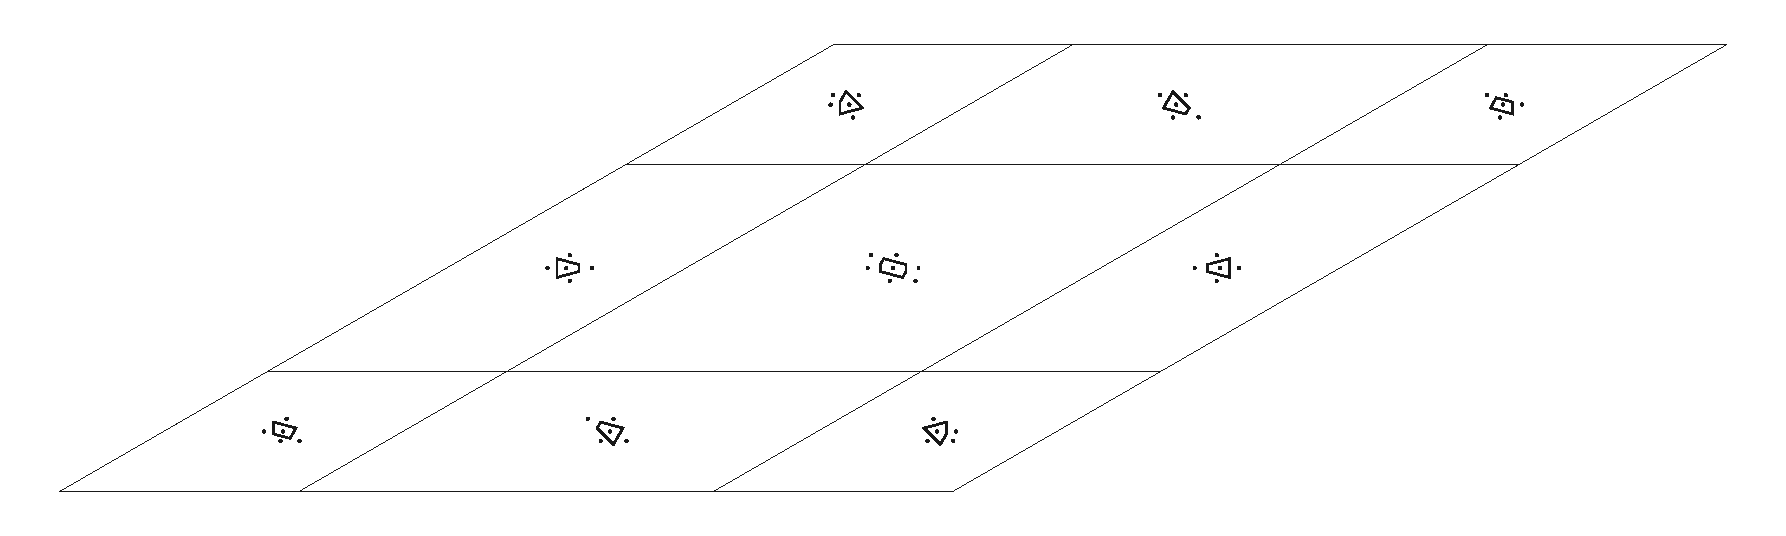
\includegraphics[width=0.96\textwidth]{catalogRhombusAll/window/window_1_4_-1_1}
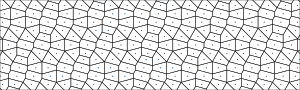
\includegraphics[width=0.96\textwidth]{catalogRhombusAll/quasi/rhombus_1_4_-1_1}
\caption*{$4-\beta$}
\end{figure}

\begin{figure}[h]
\centering
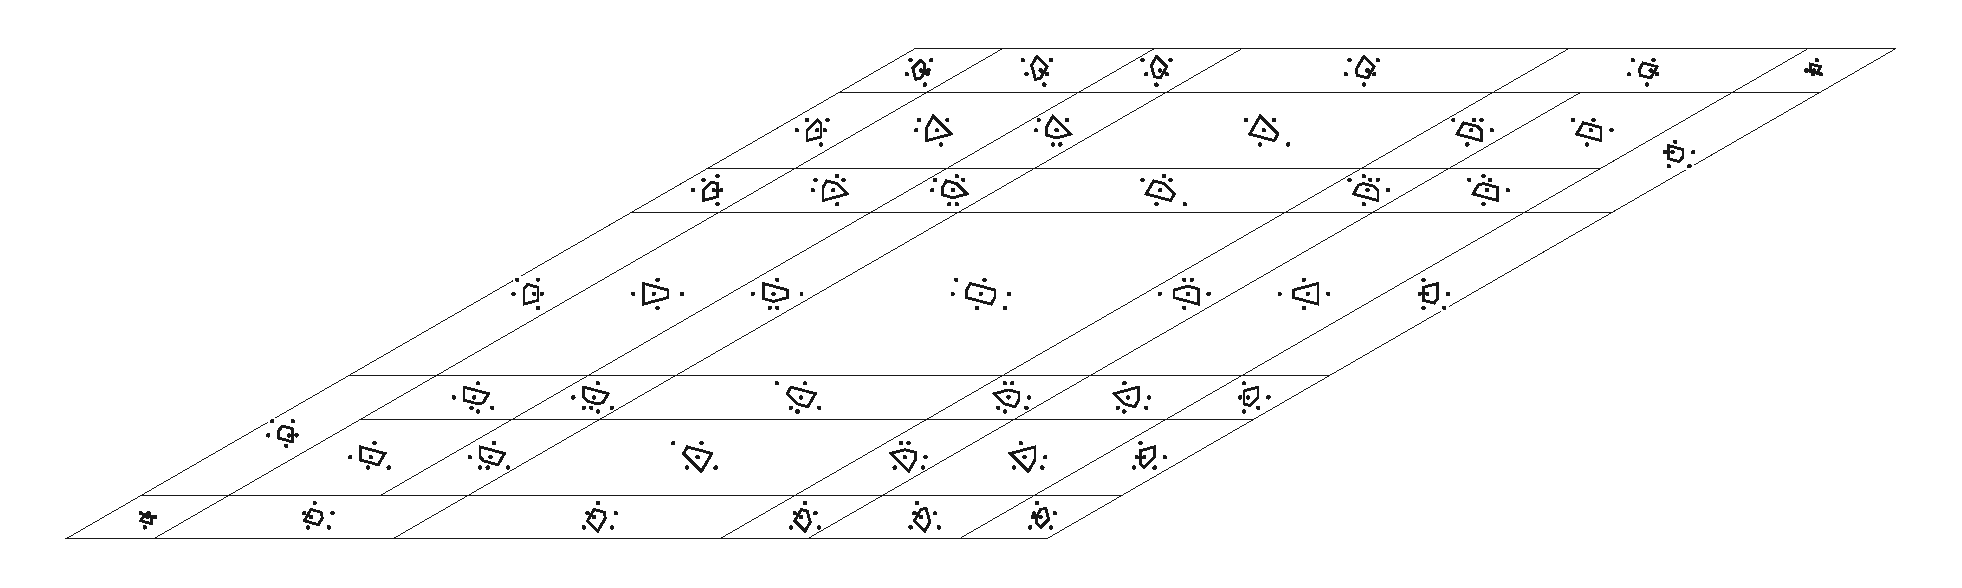
\includegraphics[width=0.96\textwidth]{catalogRhombusAll/window/window_2_-33_9_2}
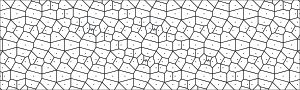
\includegraphics[width=0.96\textwidth]{catalogRhombusAll/quasi/rhombus_2_-33_9_2}
\caption*{$\frac{9\beta-33}{2}$}
\end{figure}

\begin{figure}[h]
\centering
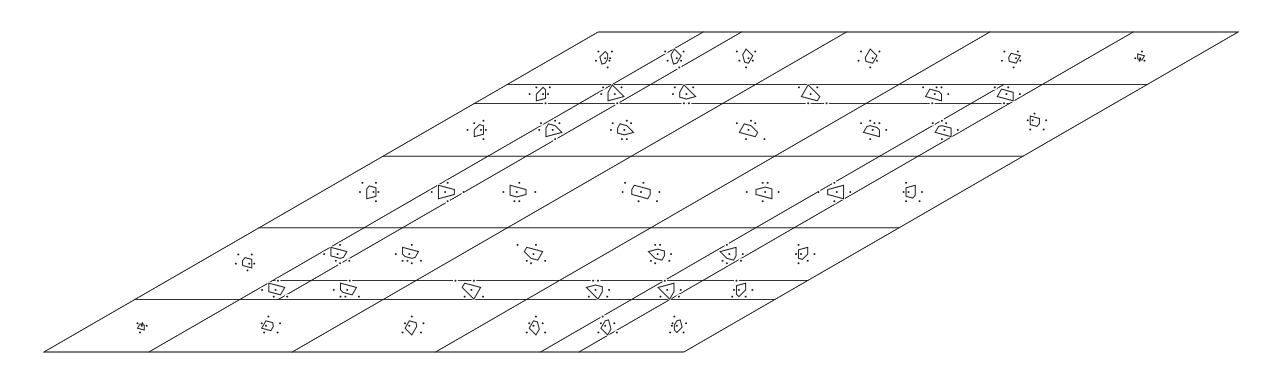
\includegraphics[width=0.96\textwidth]{catalogRhombusAll/window/window_3_-37_10_1}
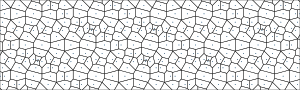
\includegraphics[width=0.96\textwidth]{catalogRhombusAll/quasi/rhombus_3_-37_10_1}
\caption*{$10\beta-37$}
\end{figure}

\begin{figure}[h]
\centering
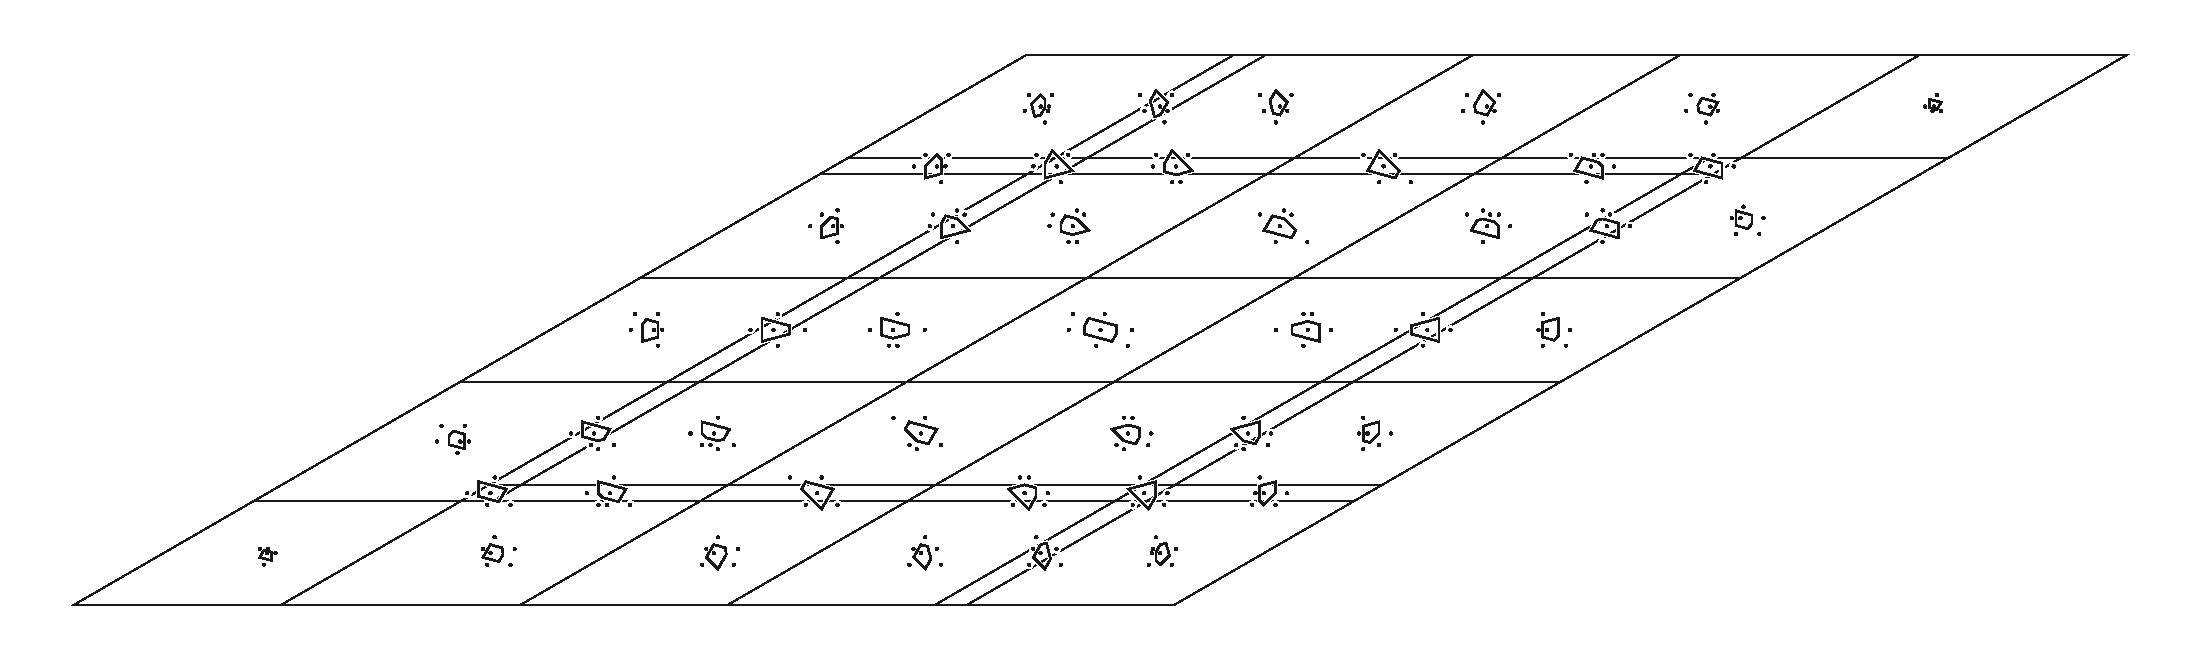
\includegraphics[width=0.96\textwidth]{catalogRhombusAll/window/window_4_-18_5_2}
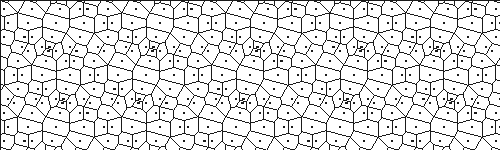
\includegraphics[width=0.96\textwidth]{catalogRhombusAll/quasi/rhombus_4_-18_5_2}
\caption*{$\frac{5\beta-18}{2}$}
\end{figure}

\begin{figure}[h]
\centering
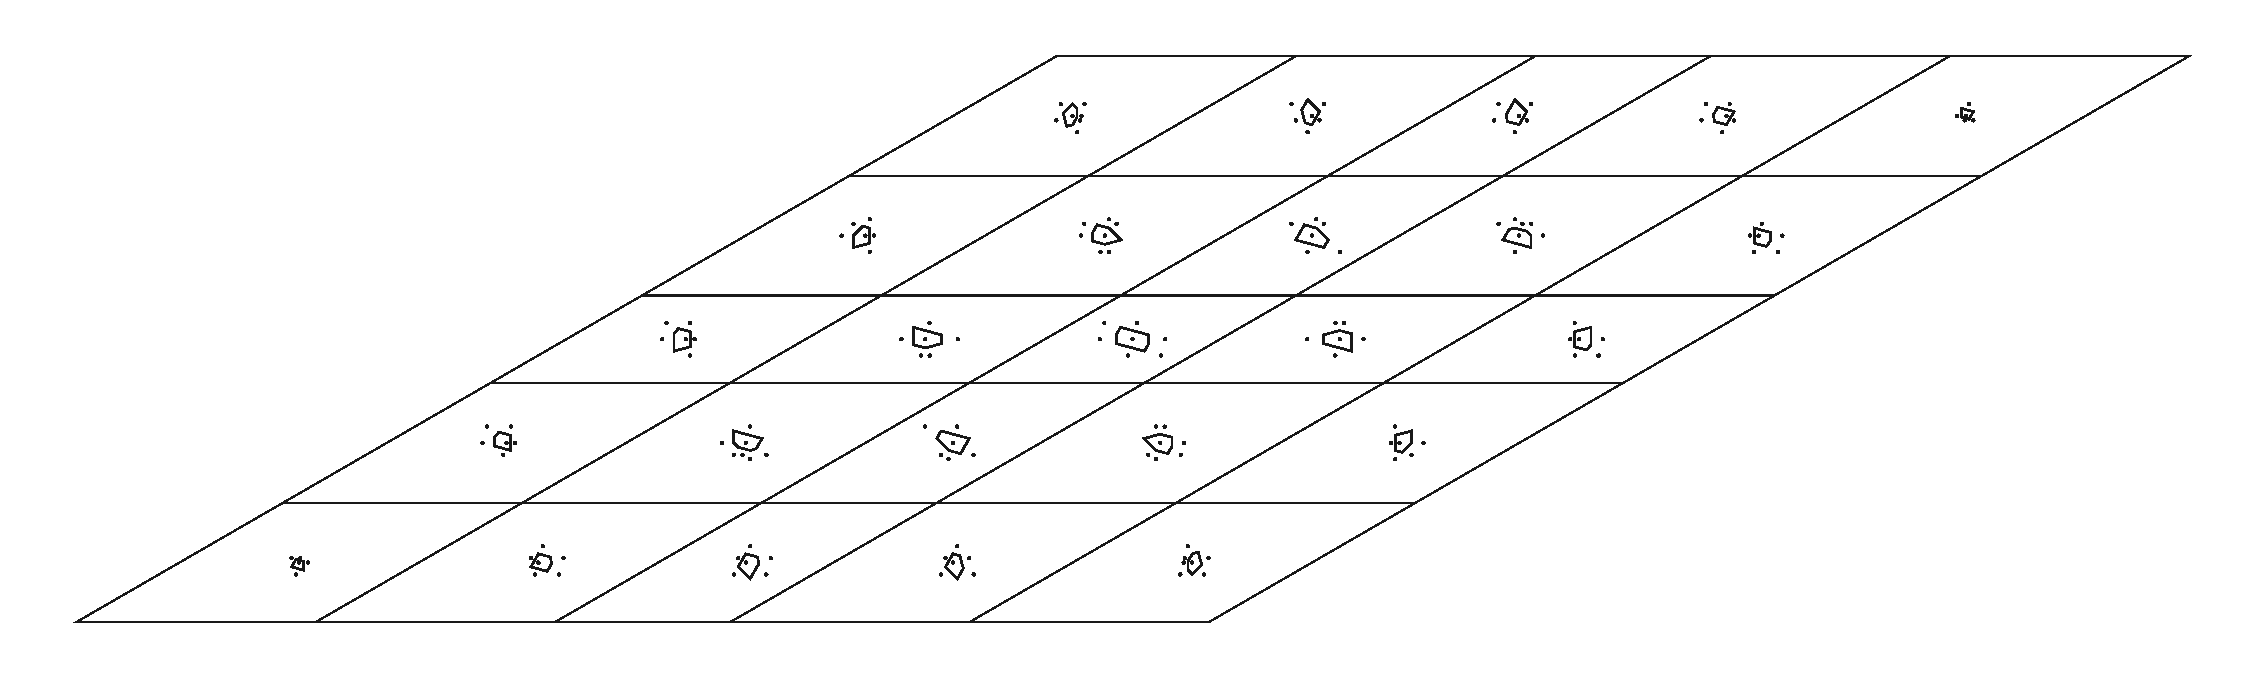
\includegraphics[width=0.96\textwidth]{catalogRhombusAll/window/window_5_19_-5_1}
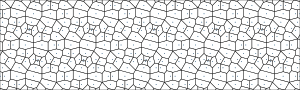
\includegraphics[width=0.96\textwidth]{catalogRhombusAll/quasi/rhombus_5_19_-5_1}
\caption*{$19-5\beta$}
\end{figure}

\thispagestyle{empty}
\begin{figure}[h]
\centering
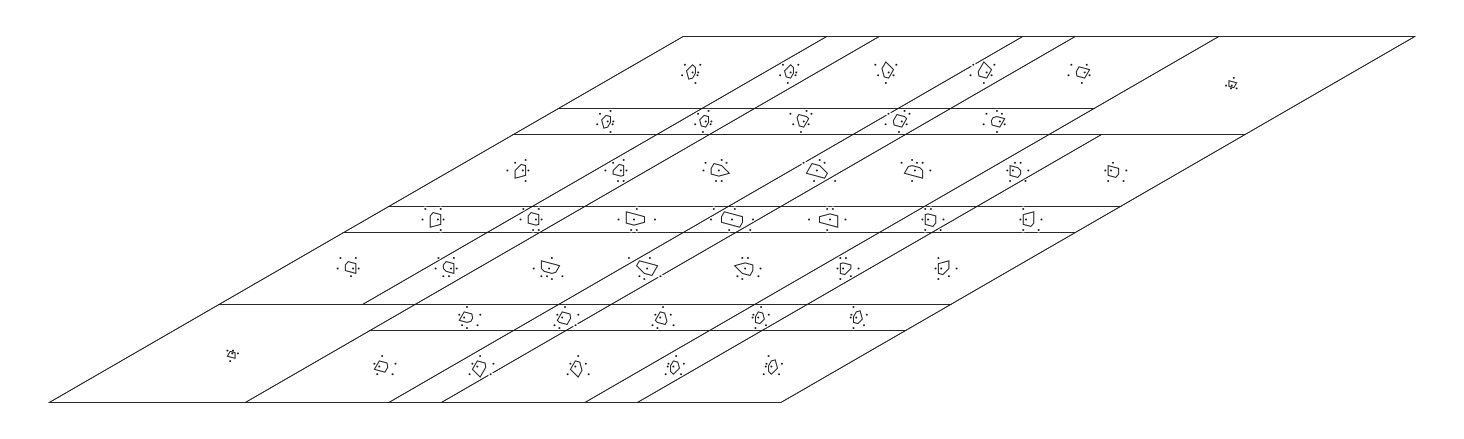
\includegraphics[width=0.96\textwidth]{catalogRhombusAll/window/window_6_-3_1_2}
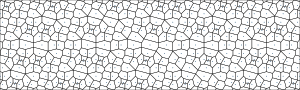
\includegraphics[width=0.96\textwidth]{catalogRhombusAll/quasi/rhombus_6_-3_1_2}
\caption*{$\frac{\beta-3}{2}$}
\end{figure}

\begin{figure}[h]
\centering
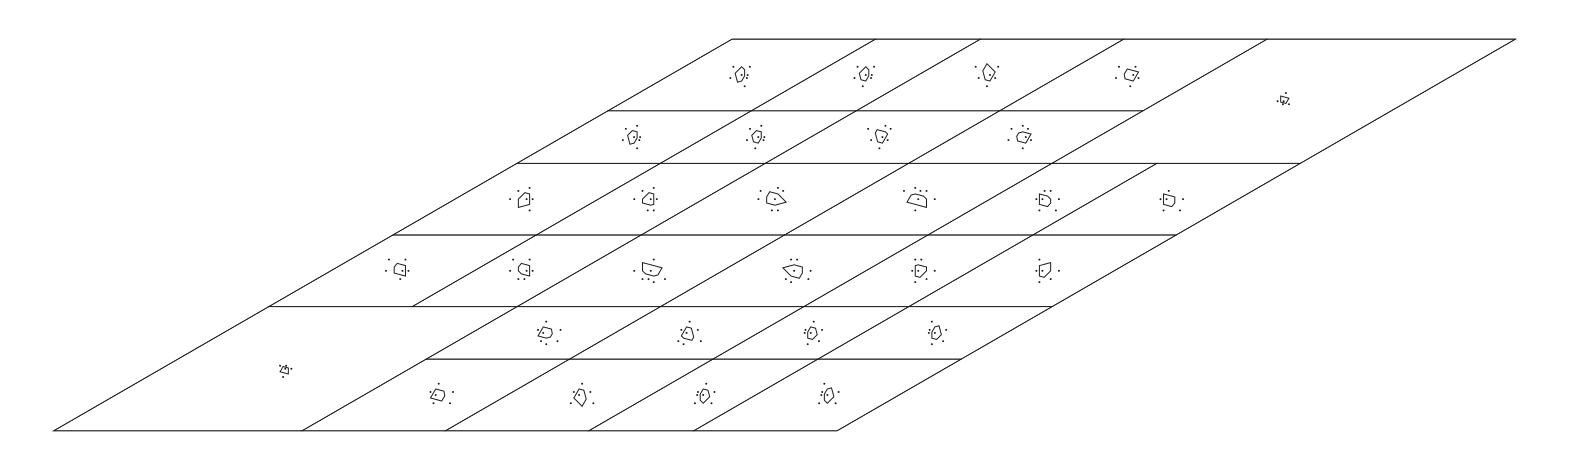
\includegraphics[width=0.96\textwidth]{catalogRhombusAll/window/window_7_-22_6_1}
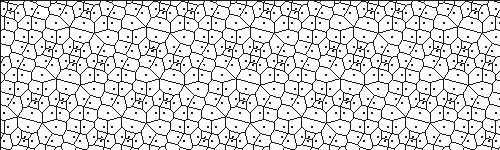
\includegraphics[width=0.96\textwidth]{catalogRhombusAll/quasi/rhombus_7_-22_6_1}
\caption*{$6\beta-22$}
\end{figure}

\begin{figure}[h]
\centering
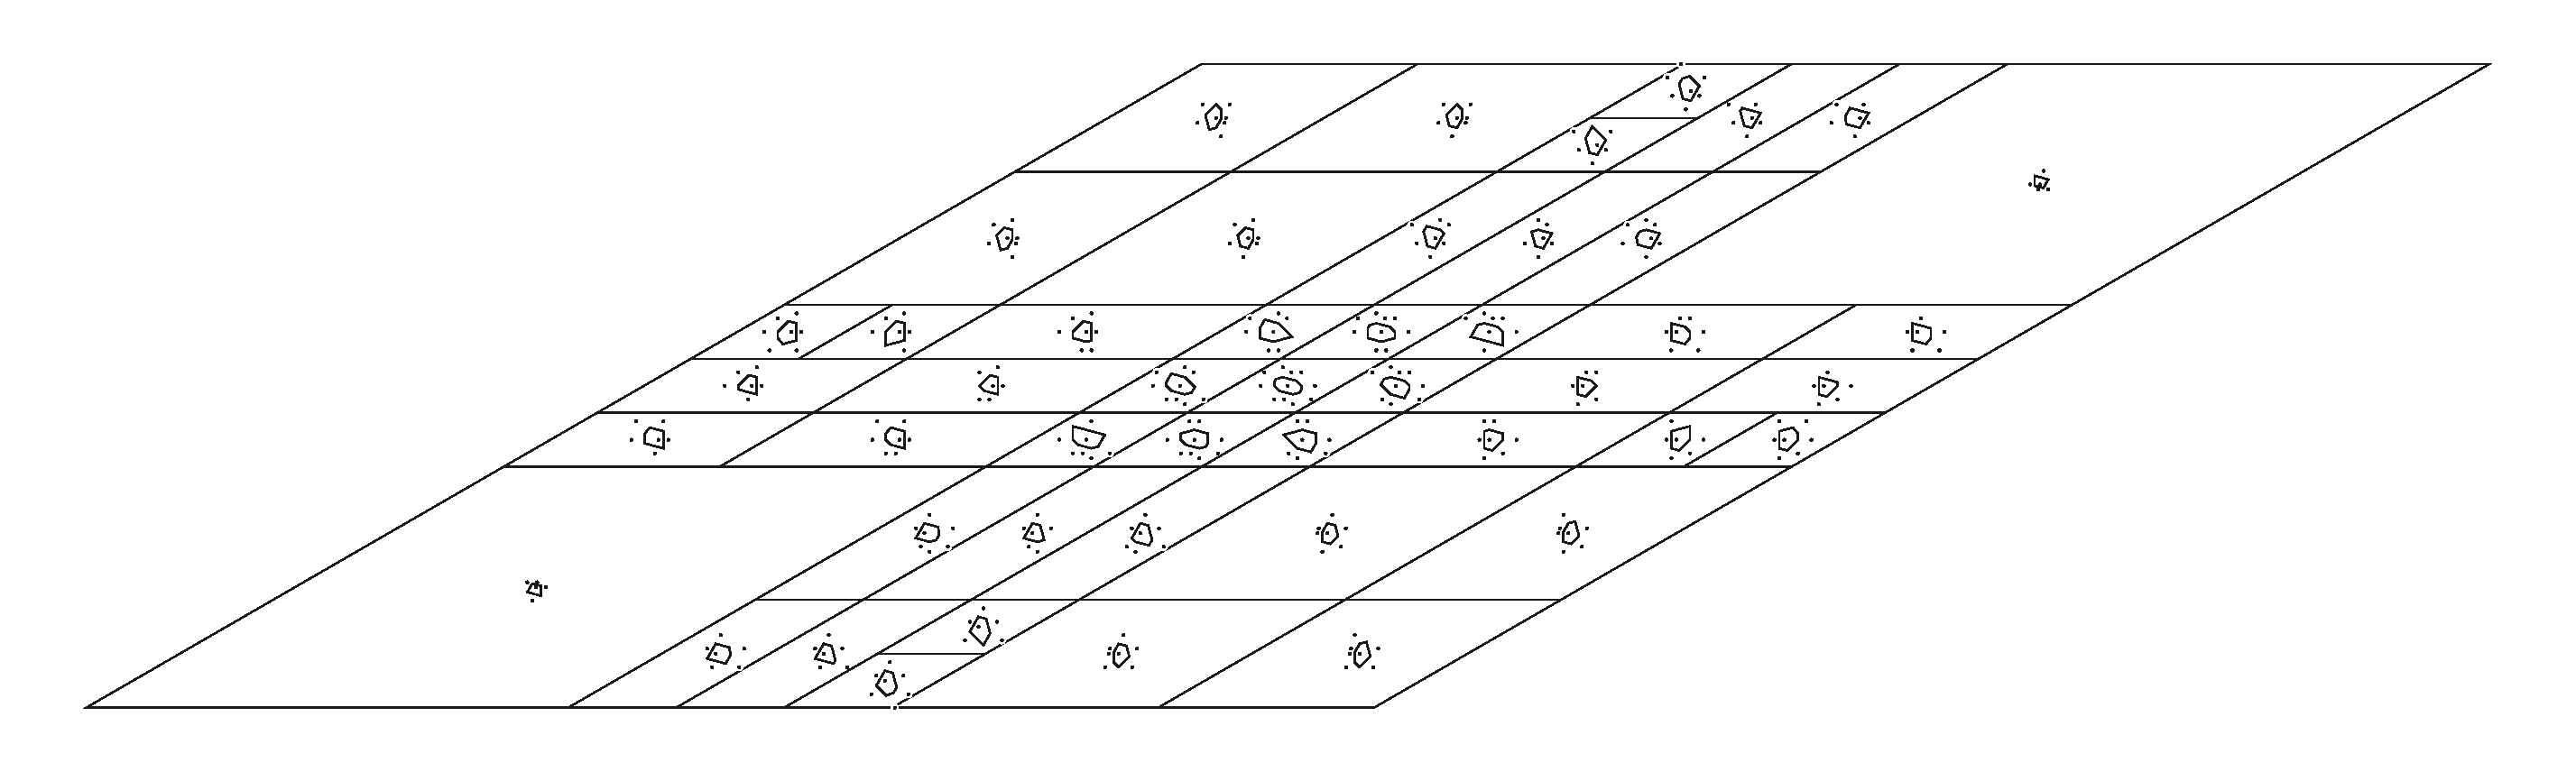
\includegraphics[width=0.96\textwidth]{catalogRhombusAll/window/window_8_-29_8_2}
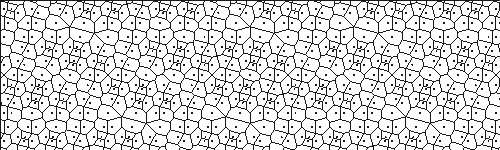
\includegraphics[width=0.96\textwidth]{catalogRhombusAll/quasi/rhombus_8_-29_8_2}
\caption*{$\frac{8\beta-29}{2}$}
\end{figure}

\begin{figure}[h]
\centering
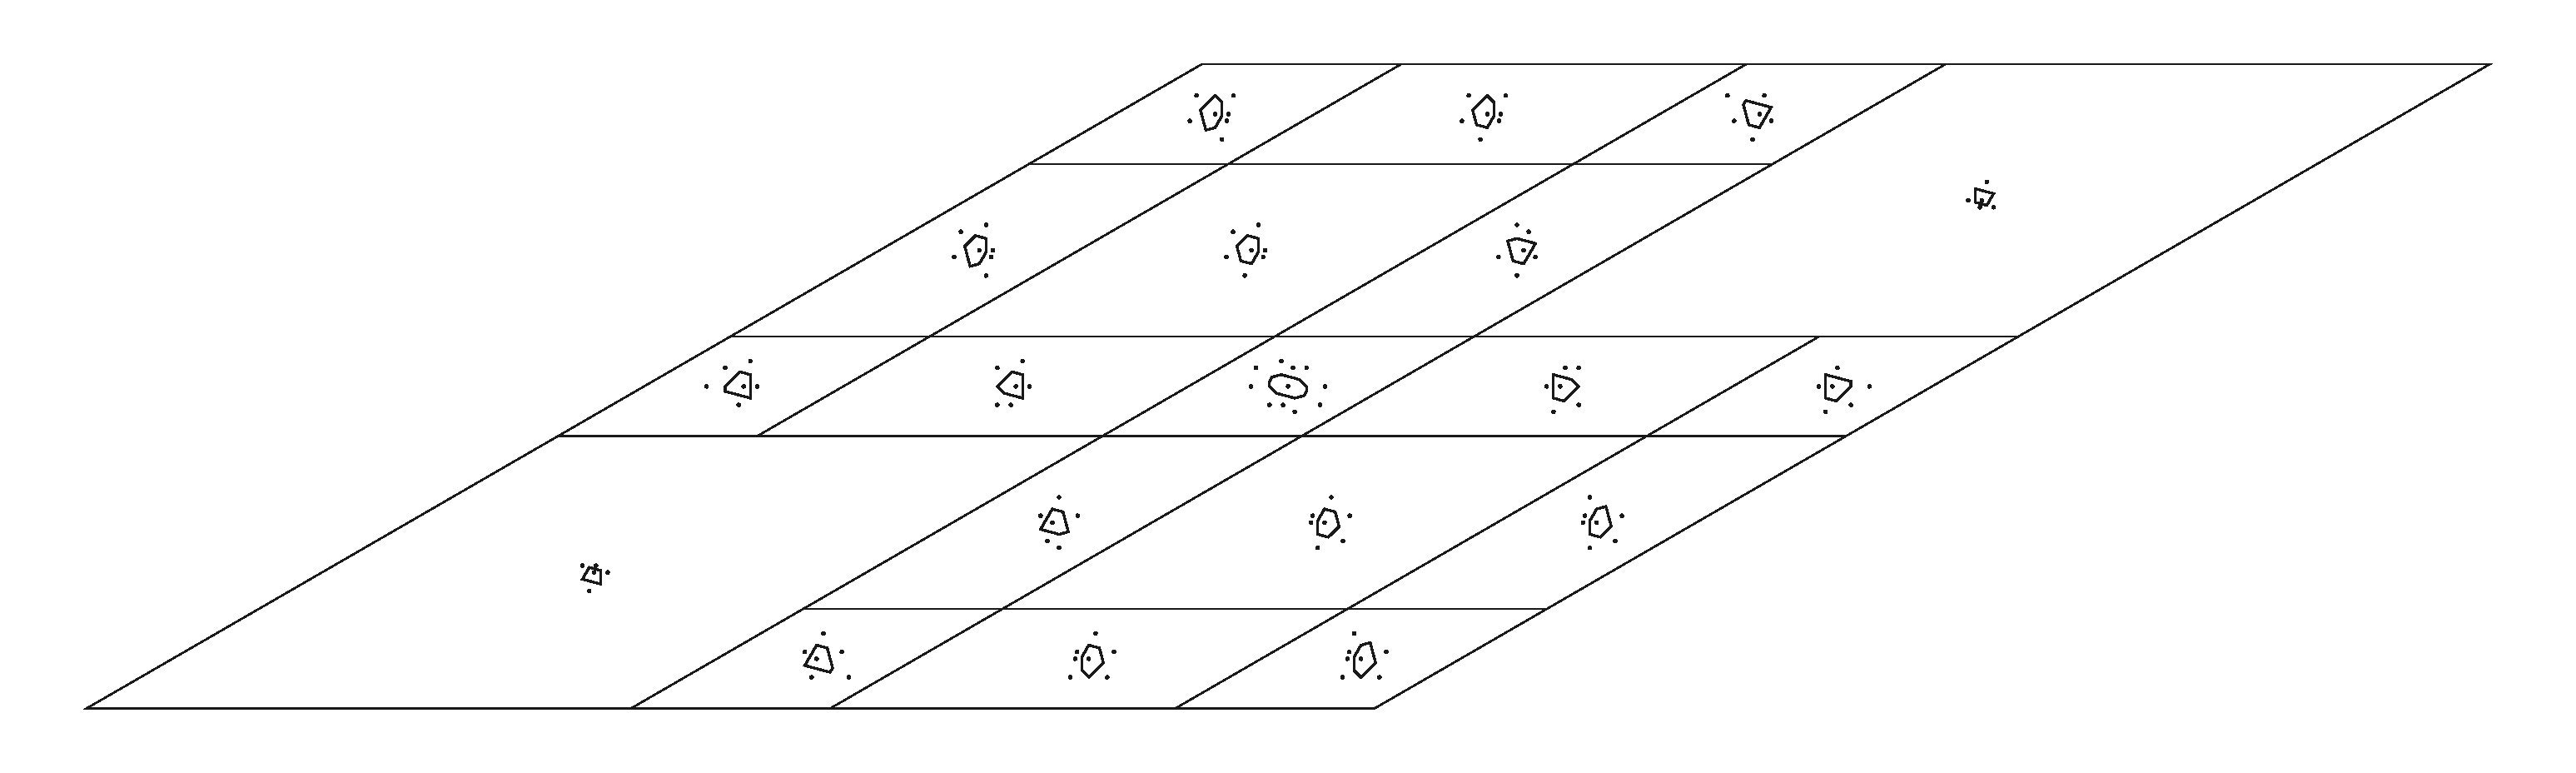
\includegraphics[width=0.96\textwidth]{catalogRhombusAll/window/window_9_-7_2_1}
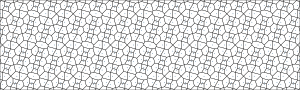
\includegraphics[width=0.96\textwidth]{catalogRhombusAll/quasi/rhombus_9_-7_2_1}
\caption*{$2\beta-7$}
\end{figure}

\begin{figure}[h]
\centering
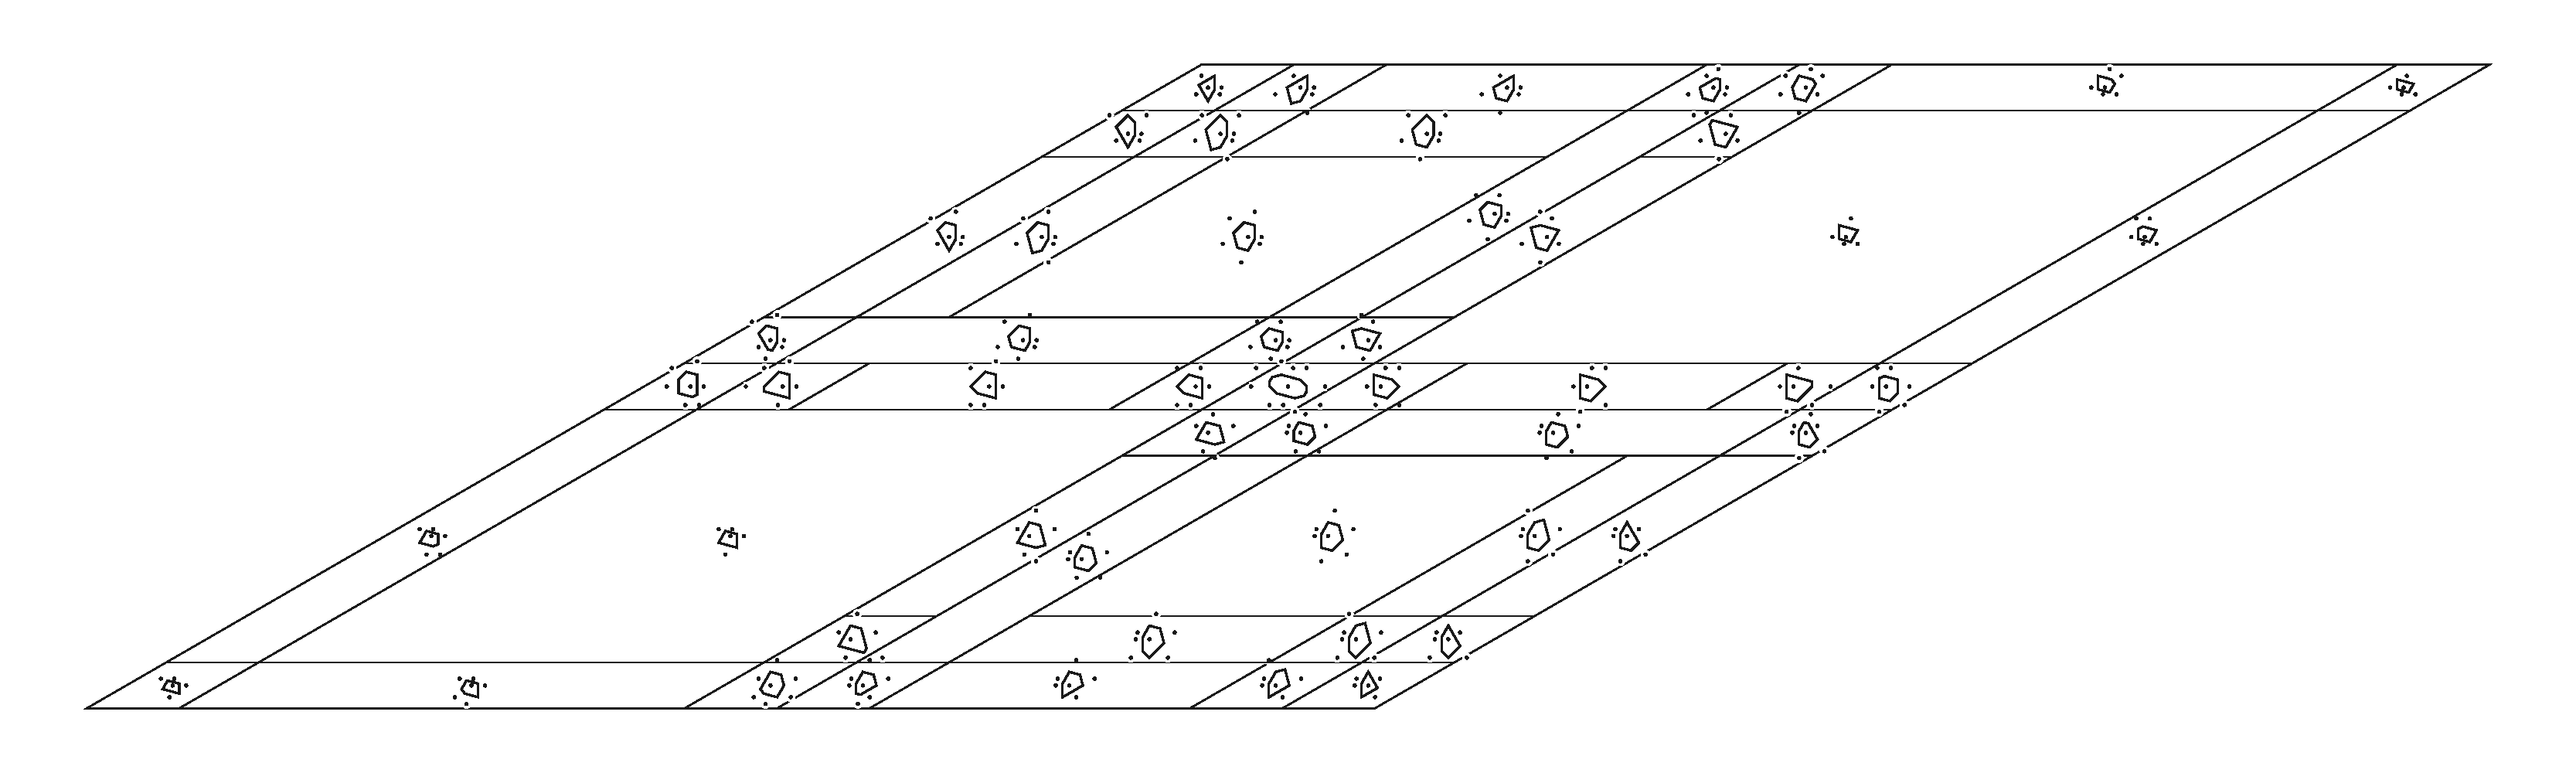
\includegraphics[width=0.96\textwidth]{catalogRhombusAll/window/window_10_1_0_2}
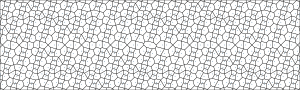
\includegraphics[width=0.96\textwidth]{catalogRhombusAll/quasi/rhombus_10_1_0_2}
\caption*{$\frac{1}{2}$}
\end{figure}

\thispagestyle{empty}
\begin{figure}[h]
\centering
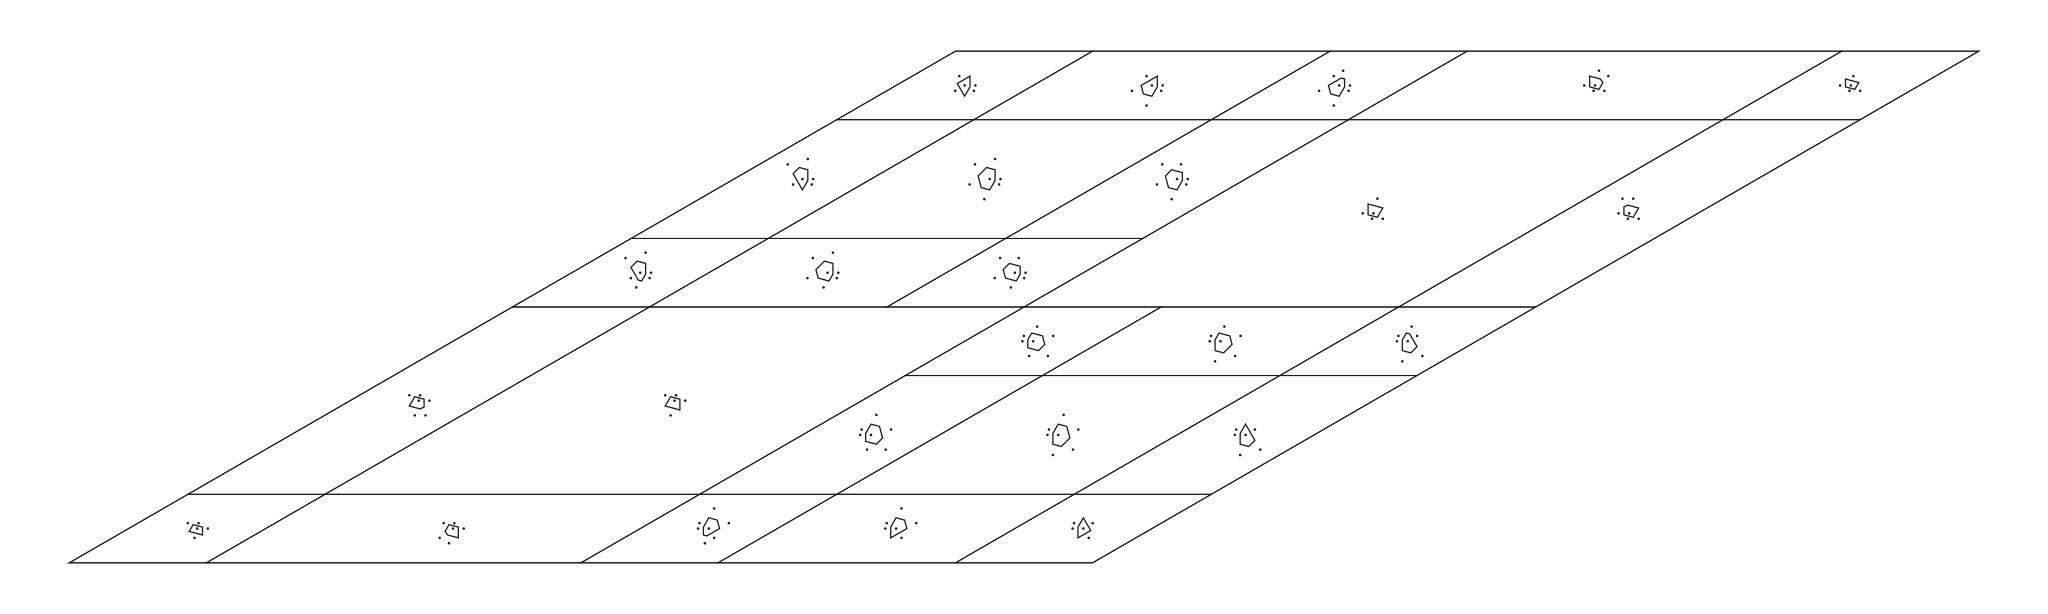
\includegraphics[width=0.96\textwidth]{catalogRhombusAll/window/window_11_8_-2_1}
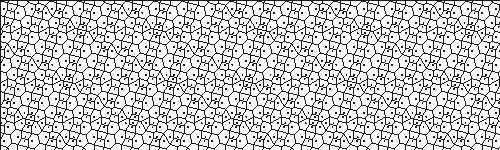
\includegraphics[width=0.96\textwidth]{catalogRhombusAll/quasi/rhombus_11_8_-2_1}
\caption*{$8-2\beta$}
\end{figure}

\begin{figure}[h]
\centering
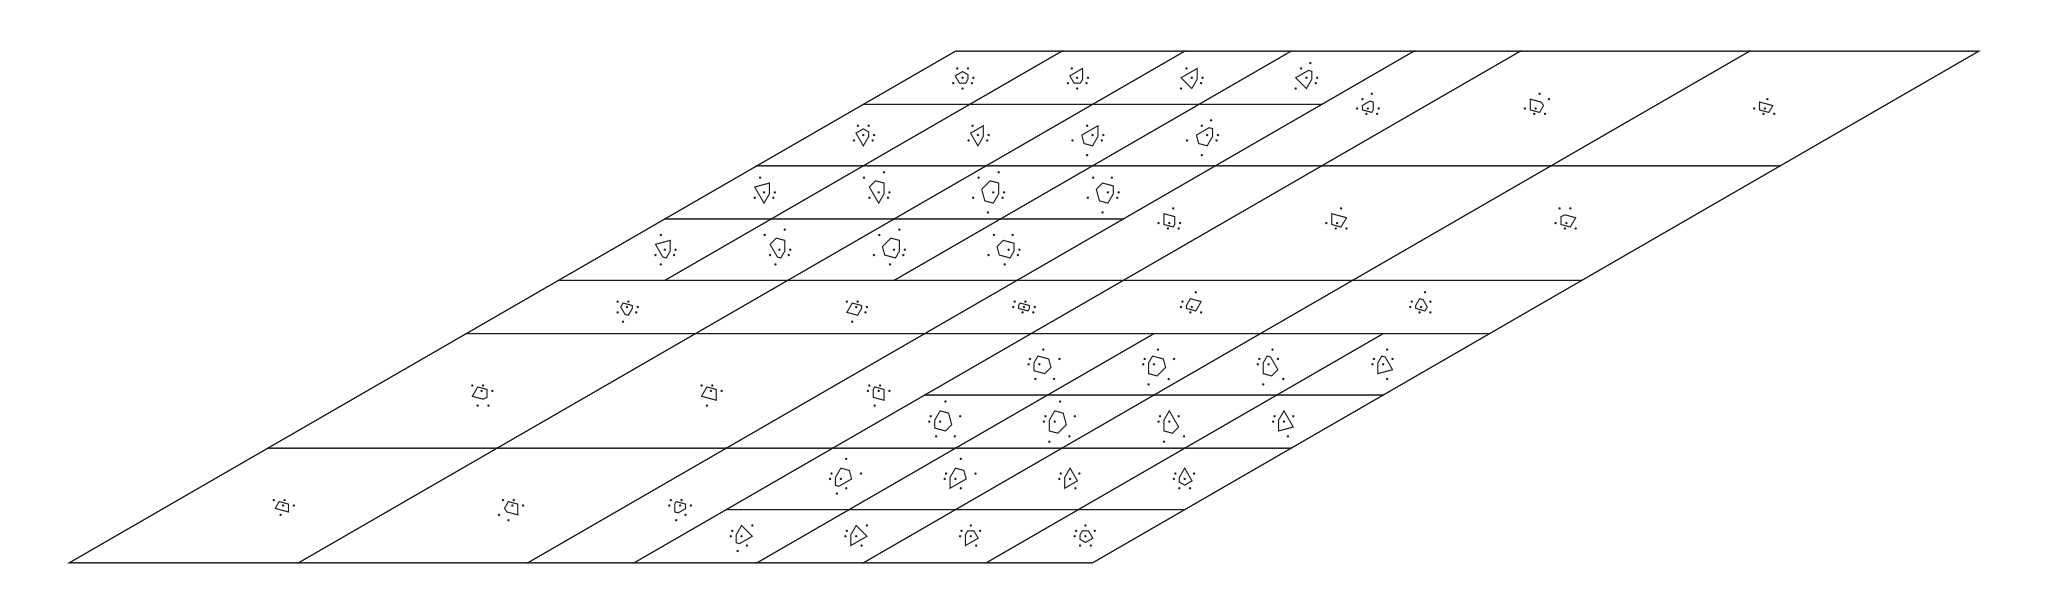
\includegraphics[width=0.96\textwidth]{catalogRhombusAll/window/window_12_-10_3_2}
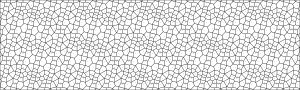
\includegraphics[width=0.96\textwidth]{catalogRhombusAll/quasi/rhombus_12_-10_3_2}
\caption*{$\frac{3\beta-10}{2}$}
\end{figure}

\begin{figure}[h]
\centering
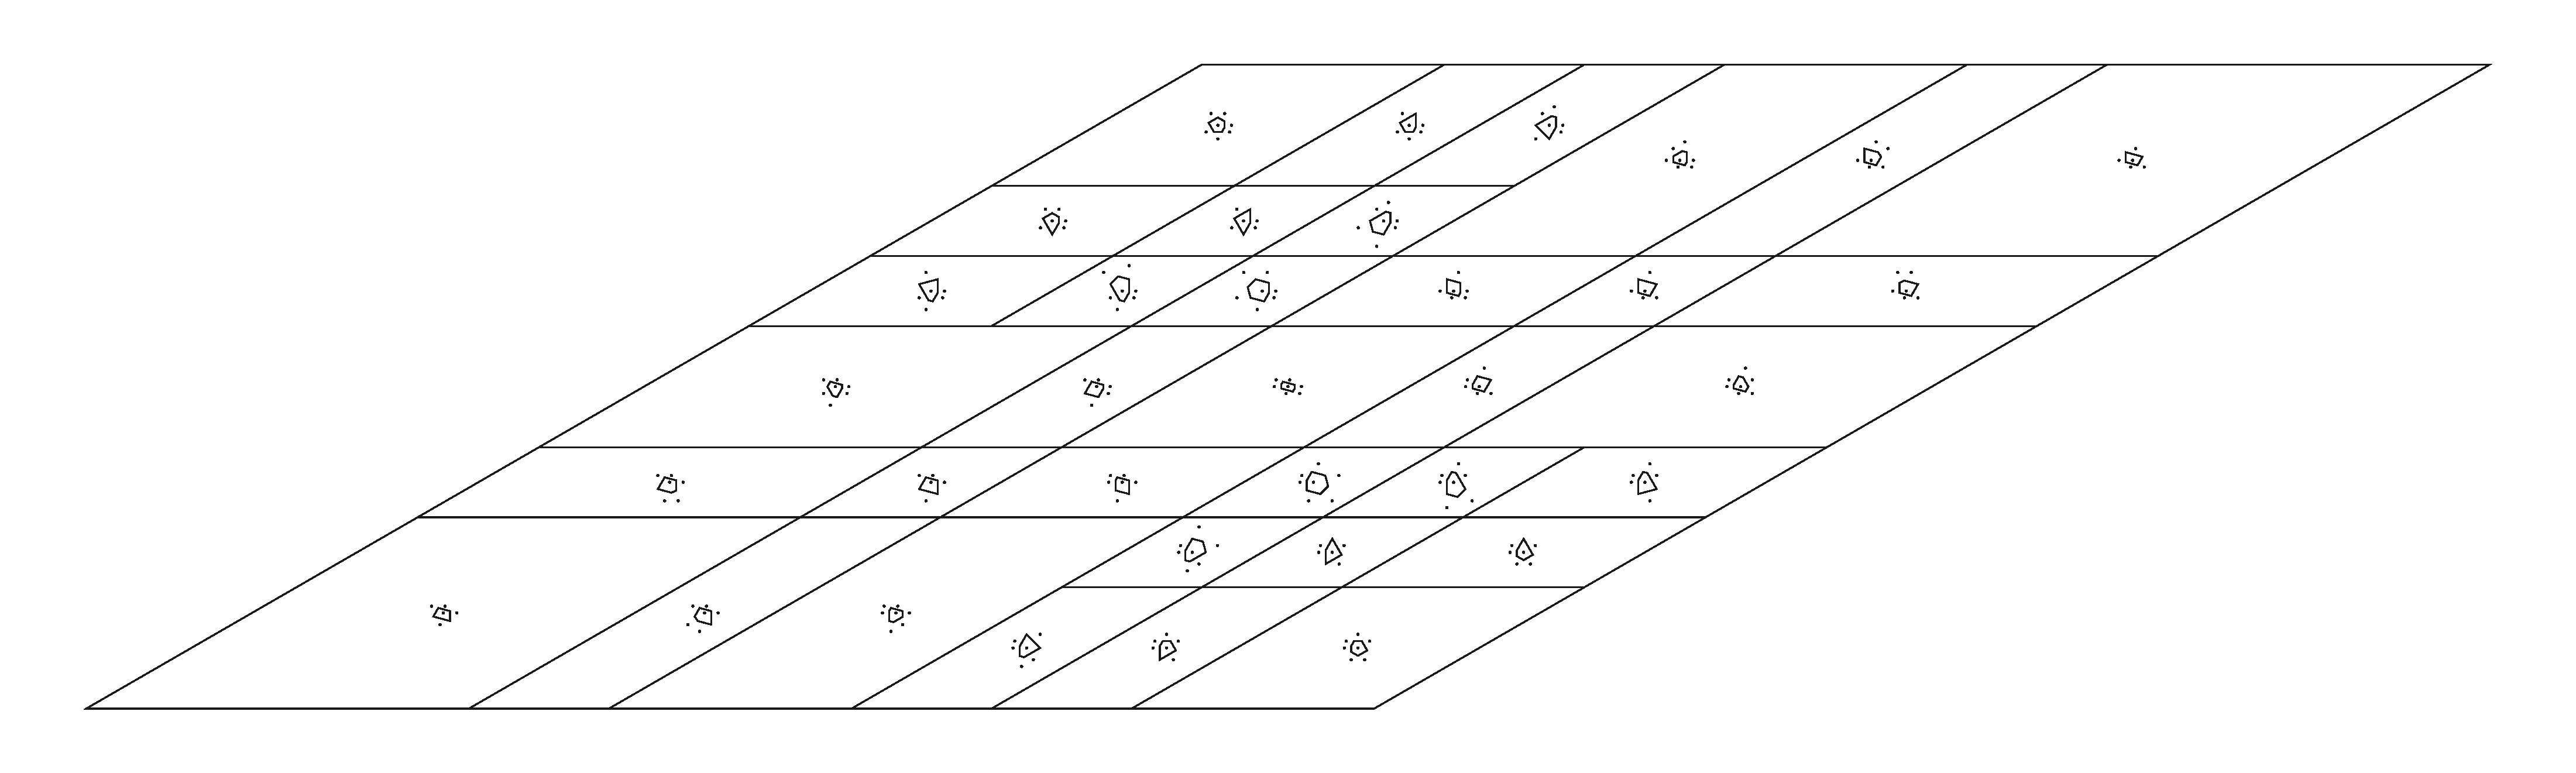
\includegraphics[width=0.96\textwidth]{catalogRhombusAll/window/window_13_-18_5_1}
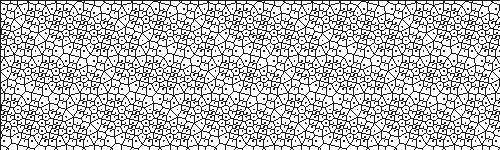
\includegraphics[width=0.96\textwidth]{catalogRhombusAll/quasi/rhombus_13_-18_5_1}
\caption*{$5\beta-18$}
\end{figure}

\begin{figure}[h]
\centering
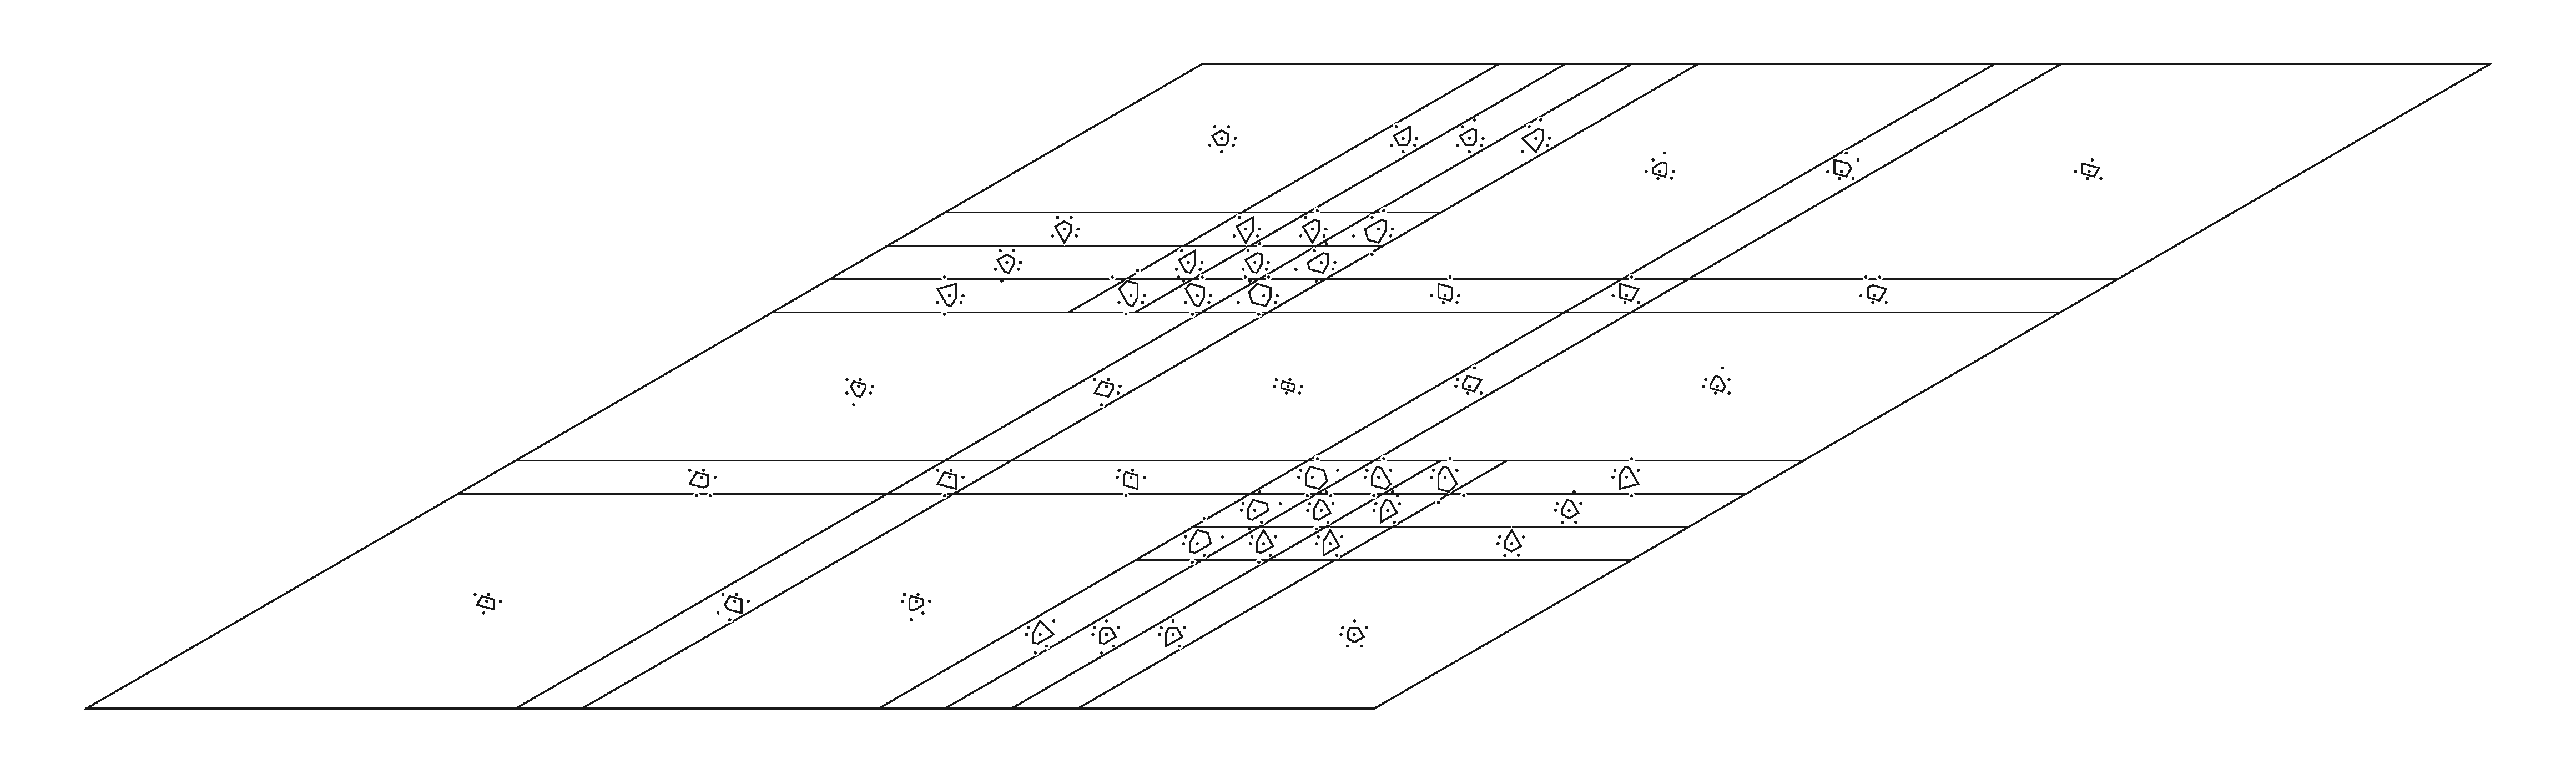
\includegraphics[width=0.96\textwidth]{catalogRhombusAll/window/window_14_-21_6_2}
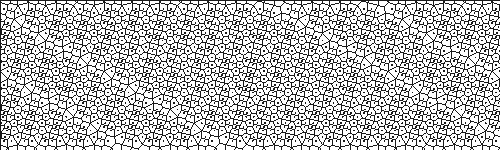
\includegraphics[width=0.96\textwidth]{catalogRhombusAll/quasi/rhombus_14_-21_6_2}
\caption*{$\frac{6\beta-21}{2}$}
\end{figure}

\begin{figure}[h]
\centering
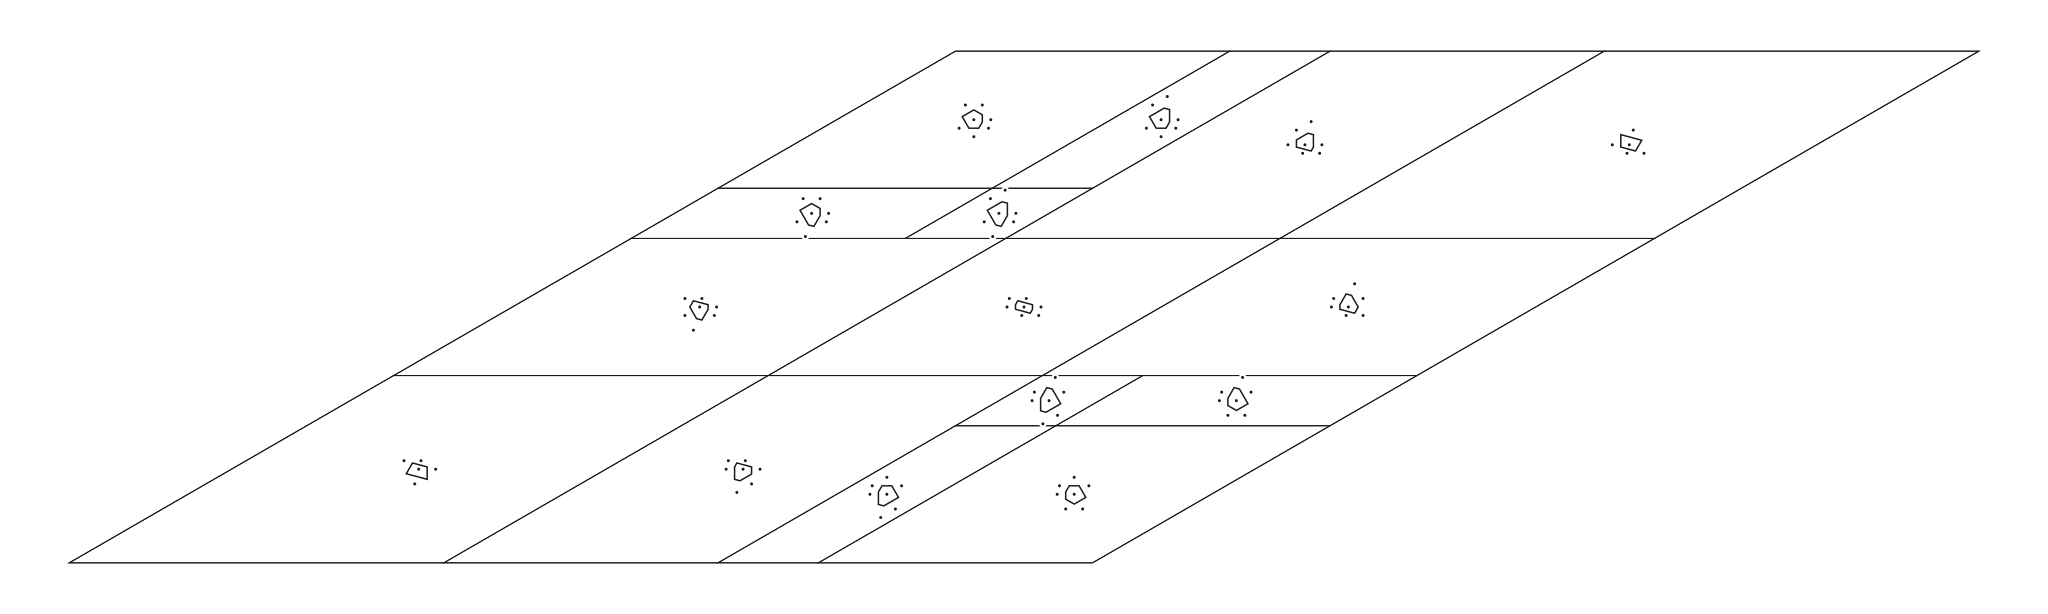
\includegraphics[width=0.96\textwidth]{catalogRhombusAll/window/window_15_-3_1_1}

\includegraphics[width=0.96\textwidth]{catalogRhombusAll/quasi/rhombus_15_-3_1_1}
\caption*{$\beta-3$}
\end{figure}

\begin{figure}[h]
\centering
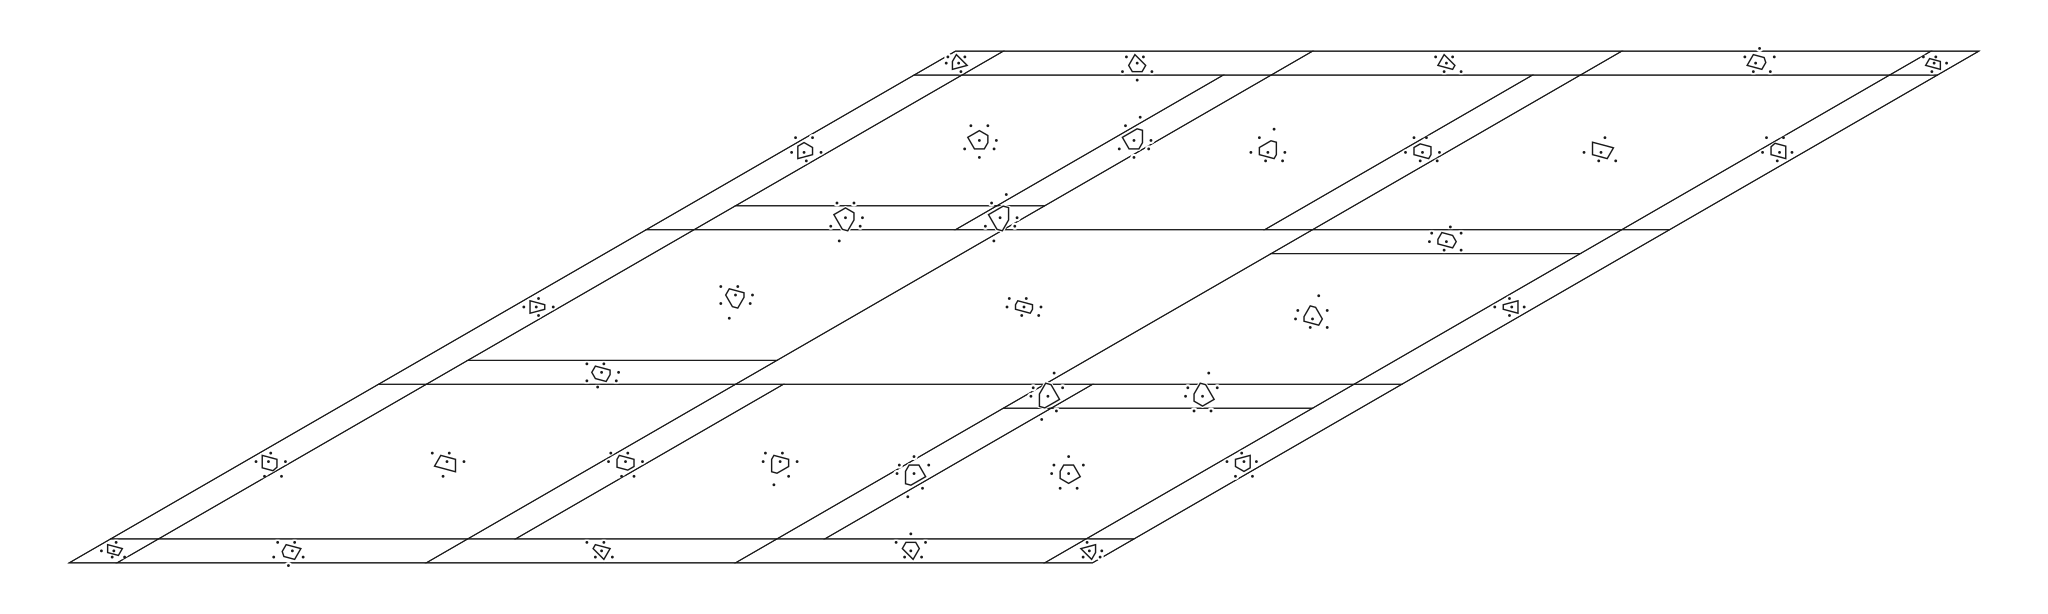
\includegraphics[width=0.96\textwidth]{catalogRhombusAll/window/window_16_9_-2_2}
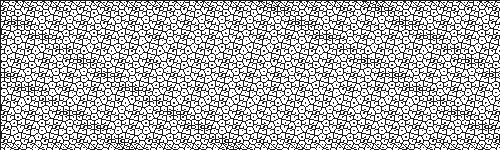
\includegraphics[width=0.96\textwidth]{catalogRhombusAll/quasi/rhombus_16_9_-2_2}
\caption*{$\frac{9-2\beta}{2}$}
\end{figure}

\begin{figure}[h]
\centering
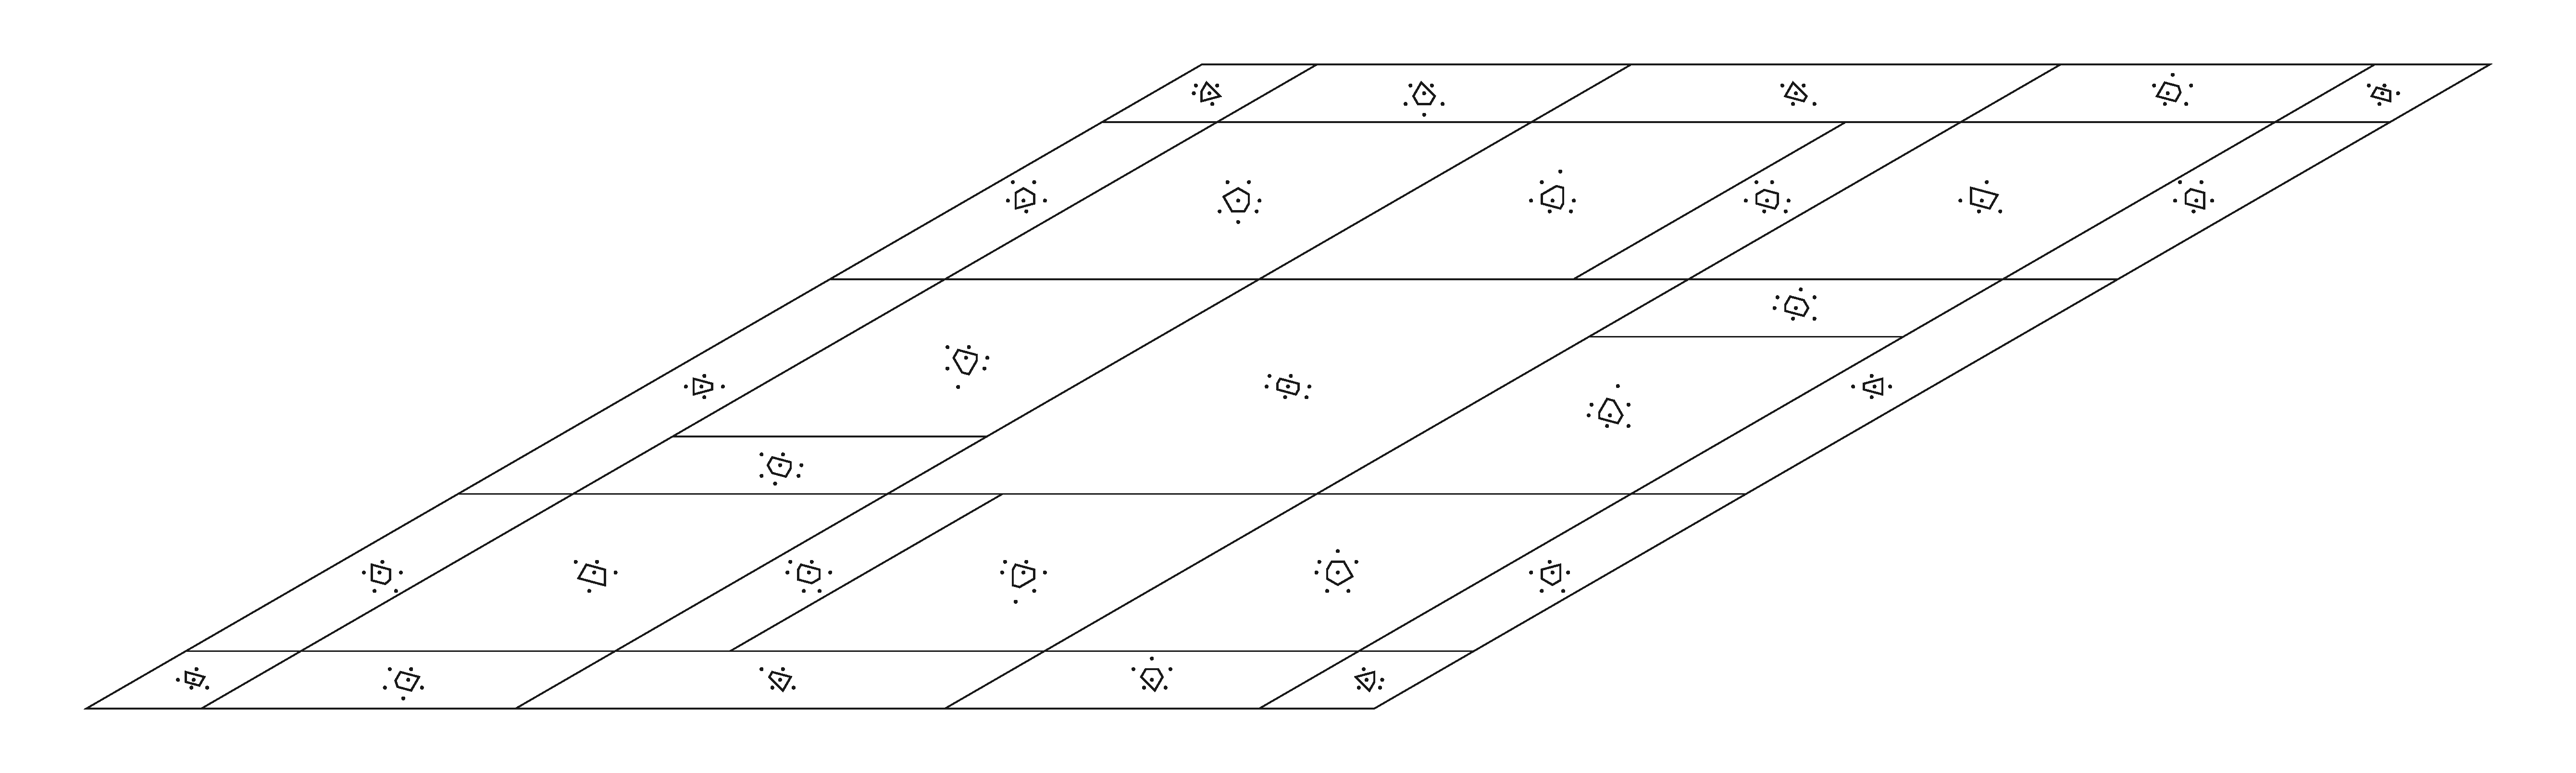
\includegraphics[width=0.96\textwidth]{catalogRhombusAll/window/window_17_12_-3_1}

\includegraphics[width=0.96\textwidth]{catalogRhombusAll/quasi/rhombus_17_12_-3_1}
\caption*{$12-3\beta$}
\end{figure}

\begin{figure}[h]
\centering
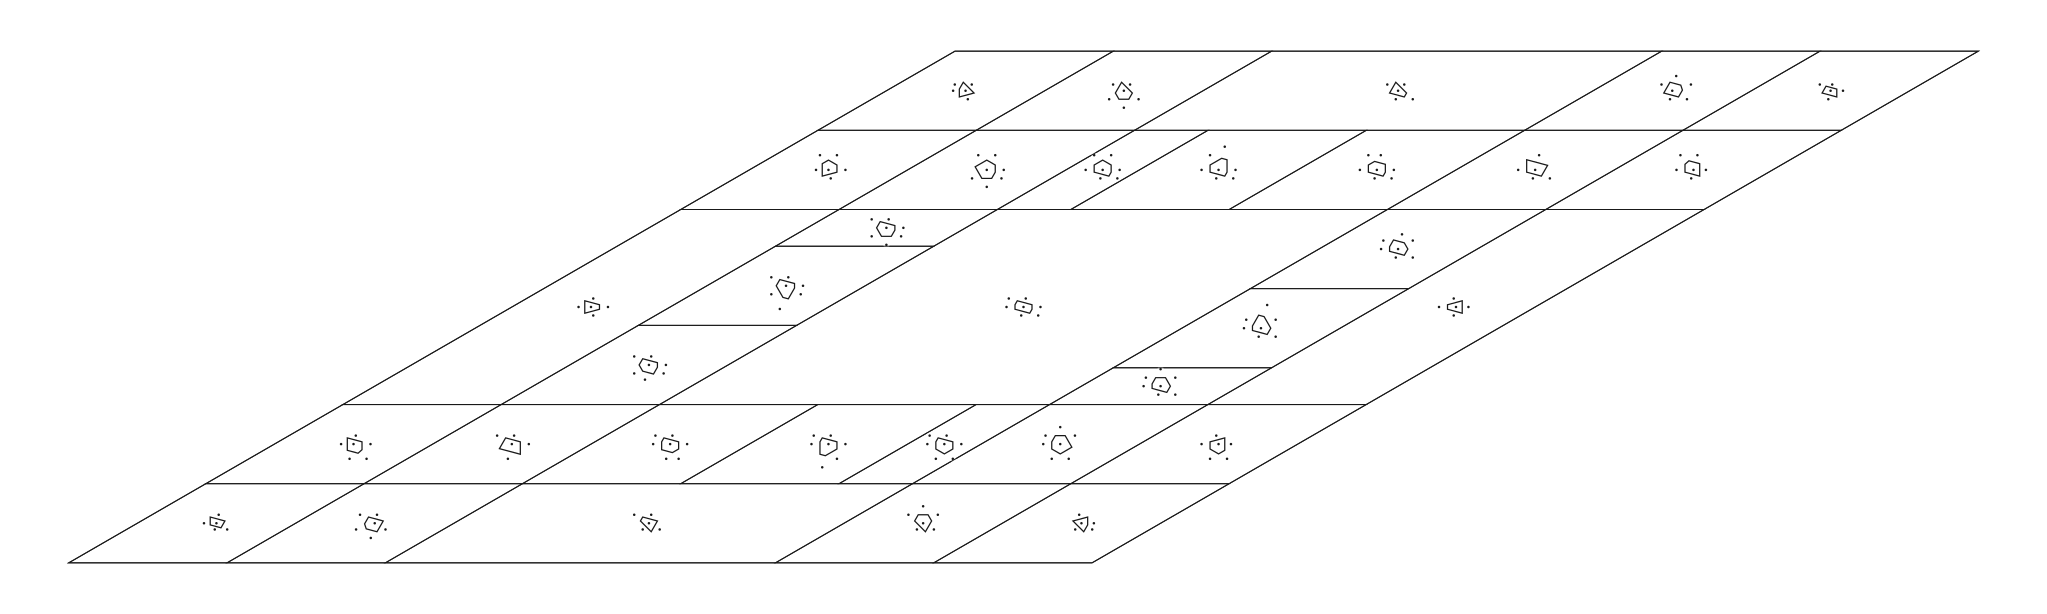
\includegraphics[width=0.96\textwidth]{catalogRhombusAll/window/window_18_-2_1_2}
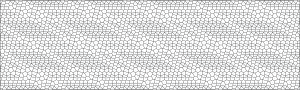
\includegraphics[width=0.96\textwidth]{catalogRhombusAll/quasi/rhombus_18_-2_1_2}
\caption*{$\frac{\beta-2}{2}$}
\end{figure}

\begin{figure}[h]
\centering
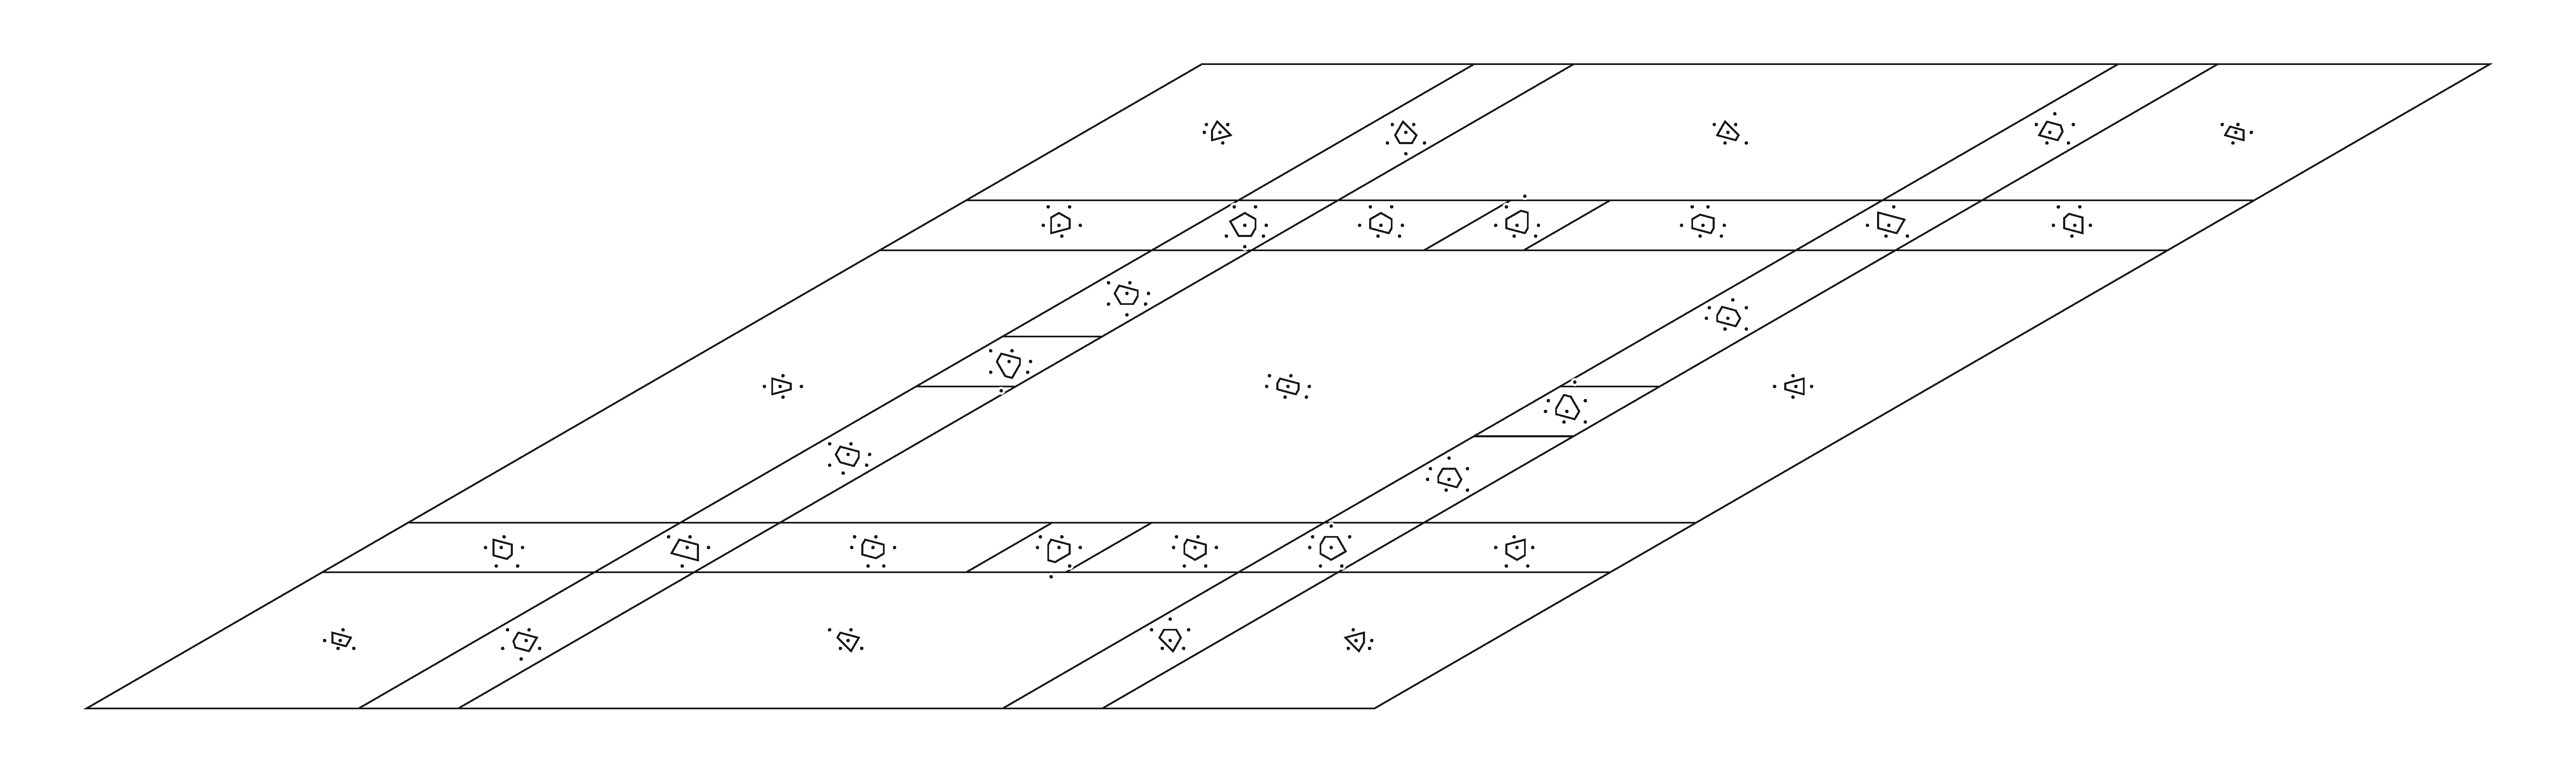
\includegraphics[width=0.96\textwidth]{catalogRhombusAll/window/window_19_-14_4_1}
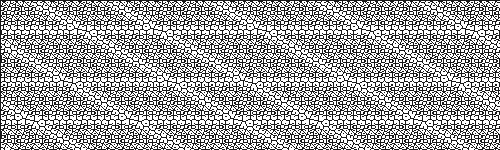
\includegraphics[width=0.96\textwidth]{catalogRhombusAll/quasi/rhombus_19_-14_4_1}
\caption*{$4\beta-14$}
\end{figure}

\begin{figure}[h]
\centering
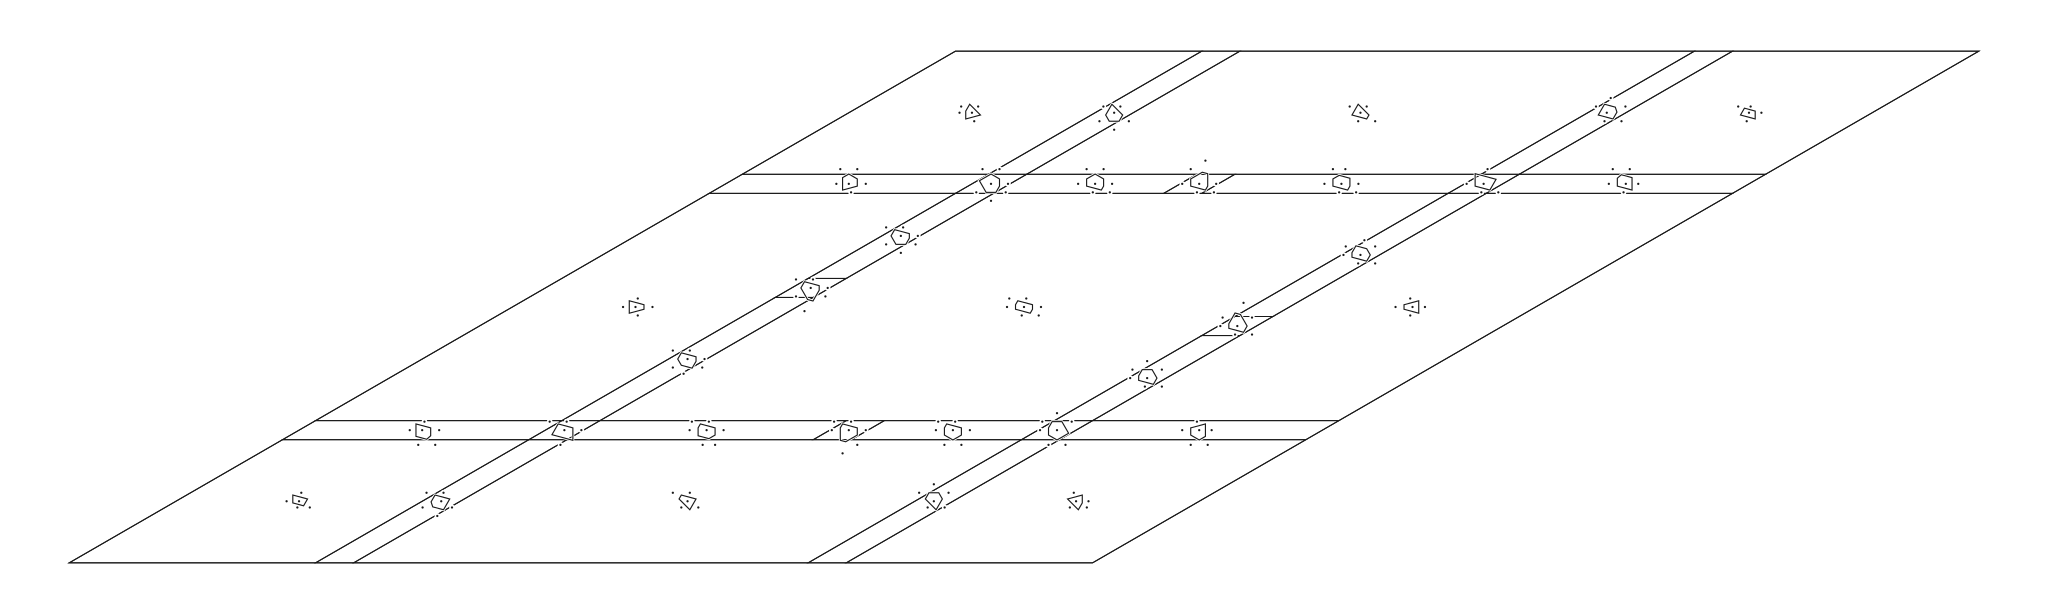
\includegraphics[width=0.96\textwidth]{catalogRhombusAll/window/window_20_-13_4_2}
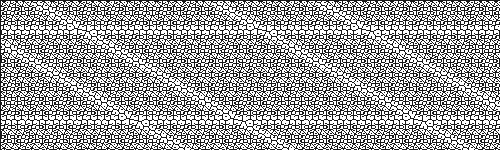
\includegraphics[width=0.96\textwidth]{catalogRhombusAll/quasi/rhombus_20_-13_4_2}
\caption*{$\frac{4\beta-13}{2}$}
\end{figure}

\begin{figure}[h]
\centering
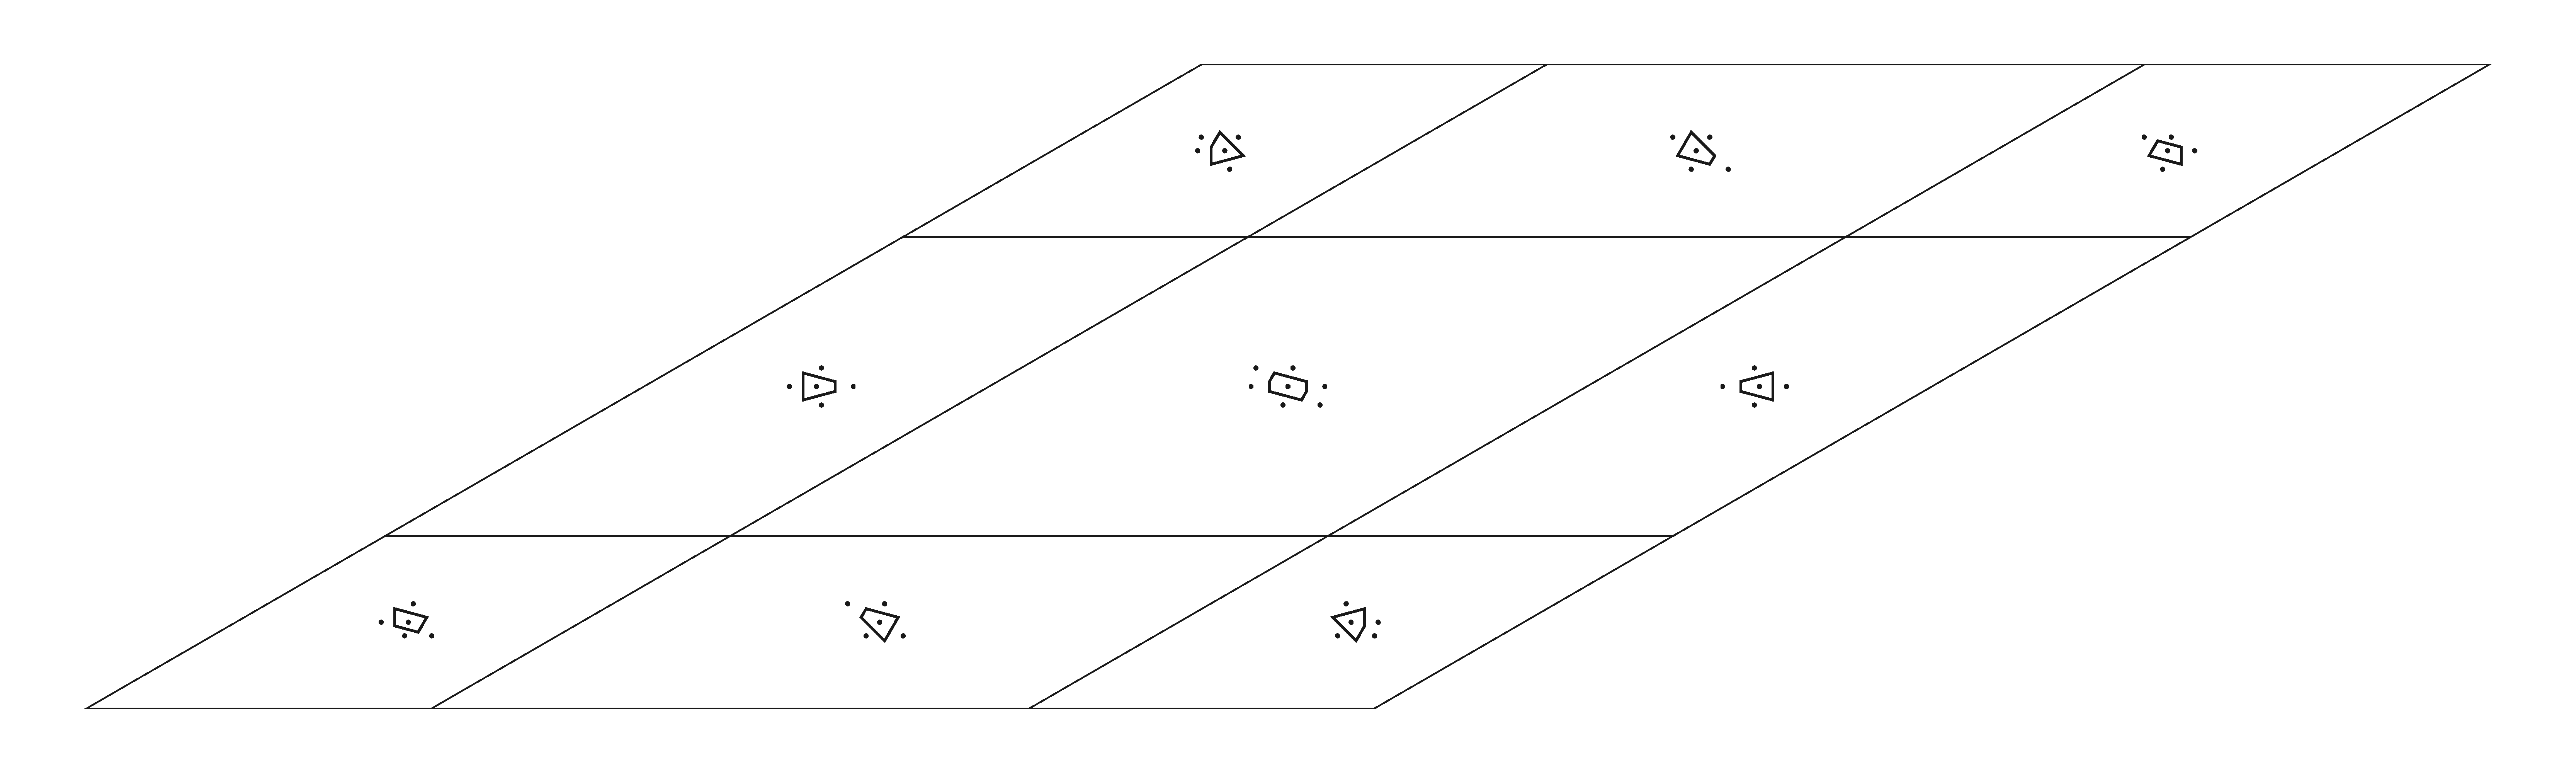
\includegraphics[width=0.96\textwidth]{catalogRhombusAll/window/window_21_1_0_1}
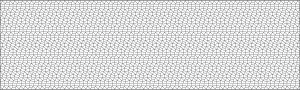
\includegraphics[width=0.96\textwidth]{catalogRhombusAll/quasi/rhombus_21_1_0_1}
\caption*{$1$}
\end{figure}
\end{landscape}

\thispagestyle{empty}
\begin{figure}[h]
\begin{flushleft}
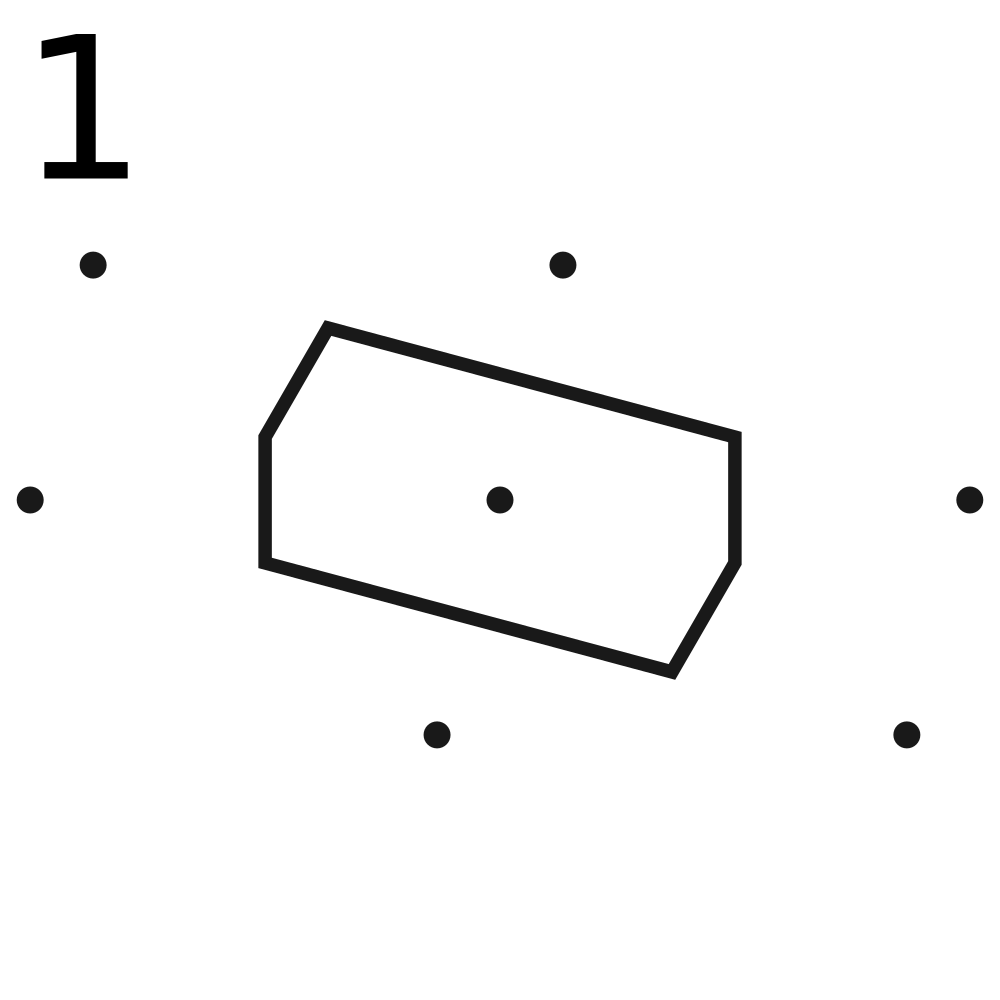
\includegraphics[scale=0.11]{catalogRhombusAll/tiles/tile001}%
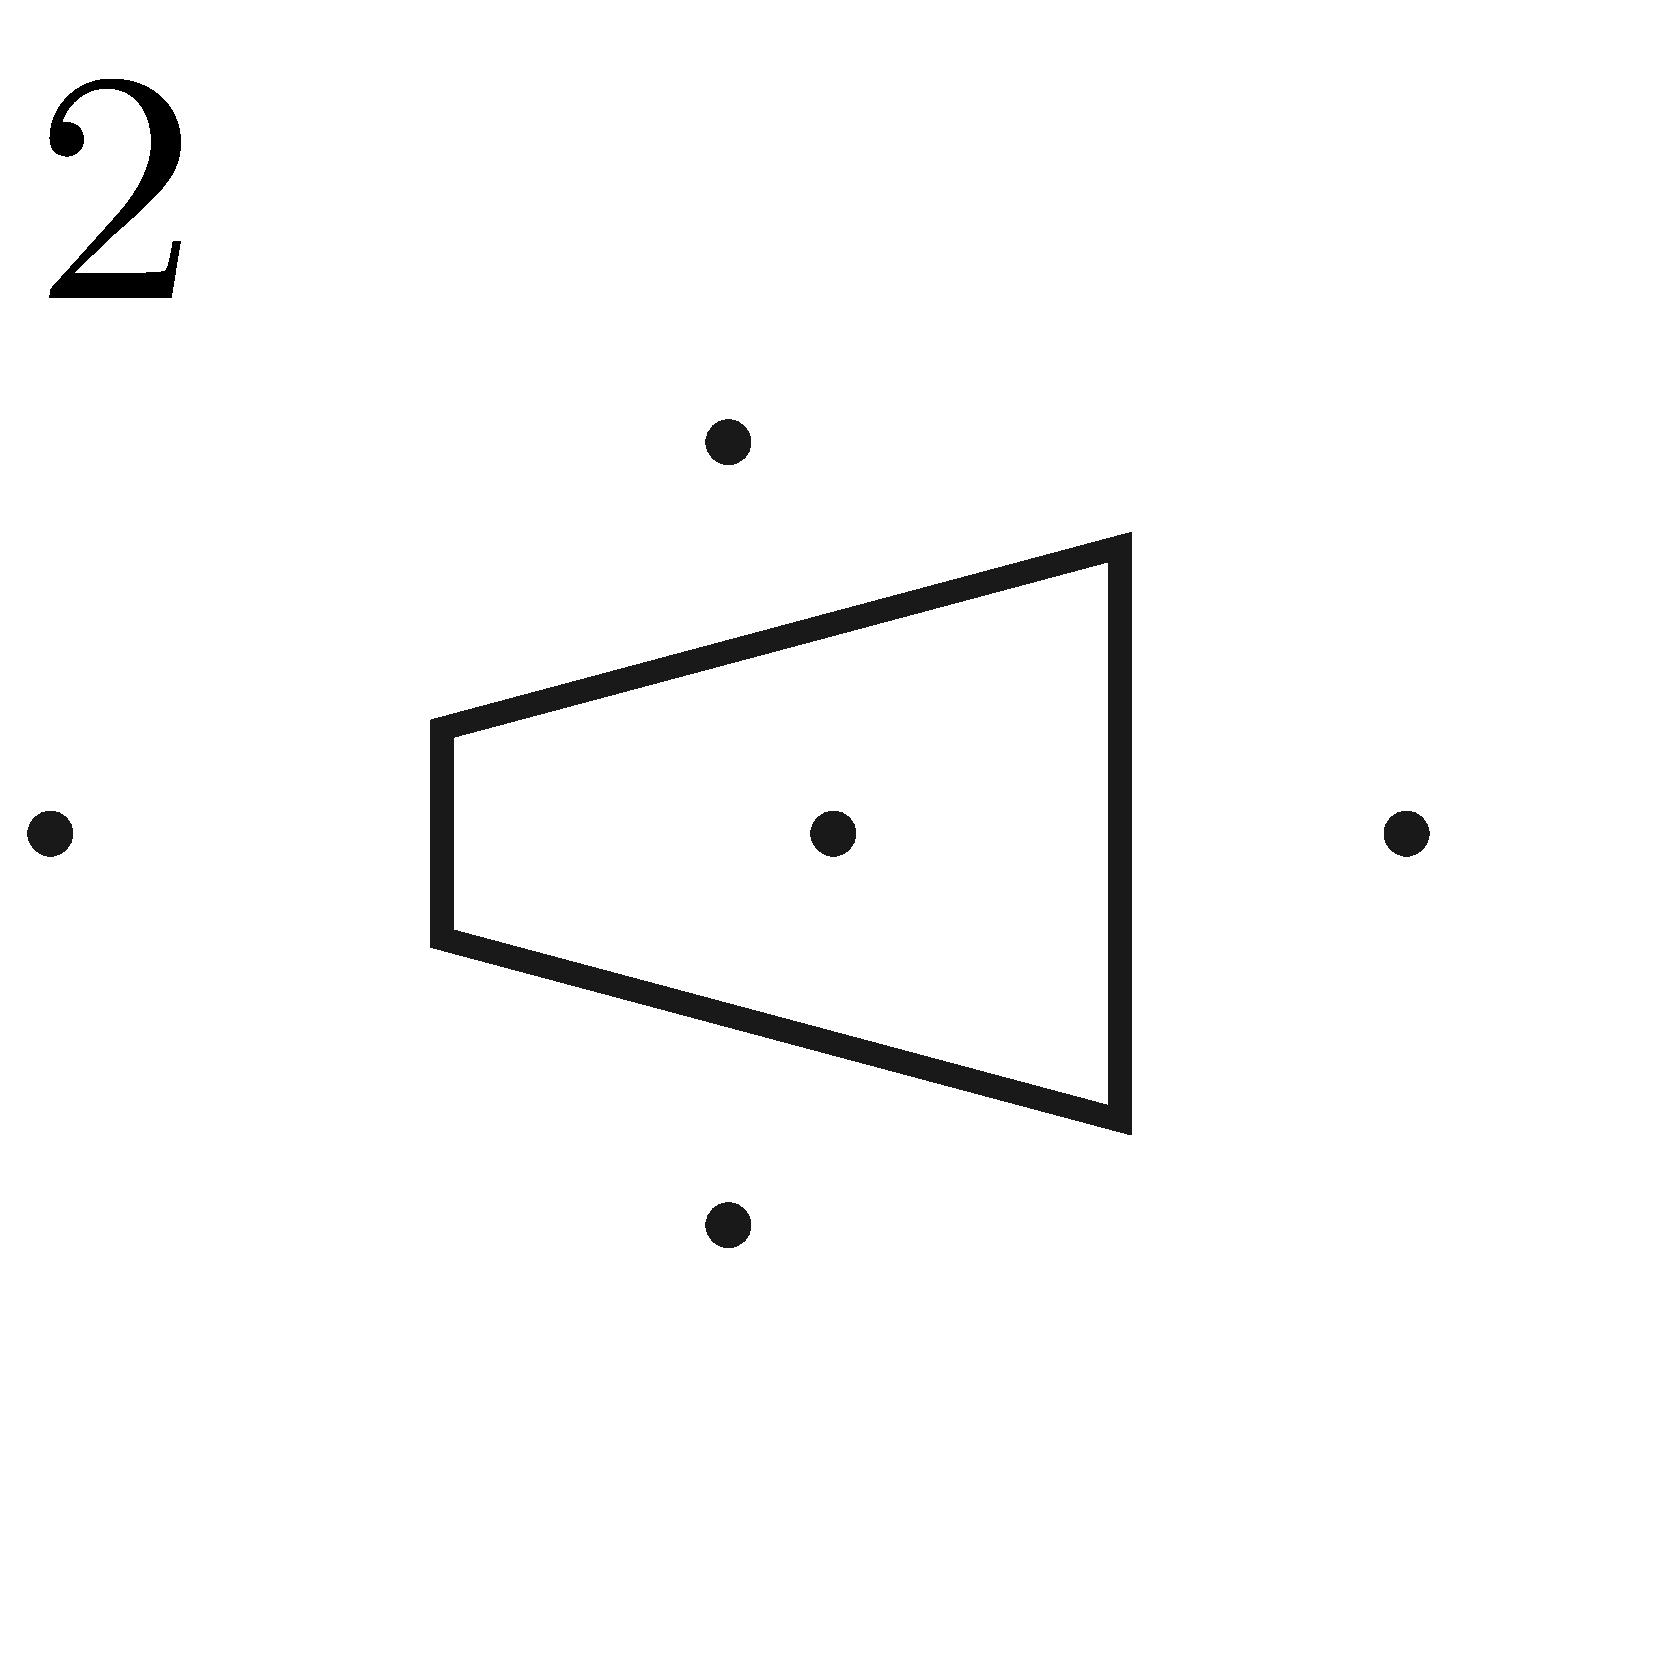
\includegraphics[scale=0.11]{catalogRhombusAll/tiles/tile002}%
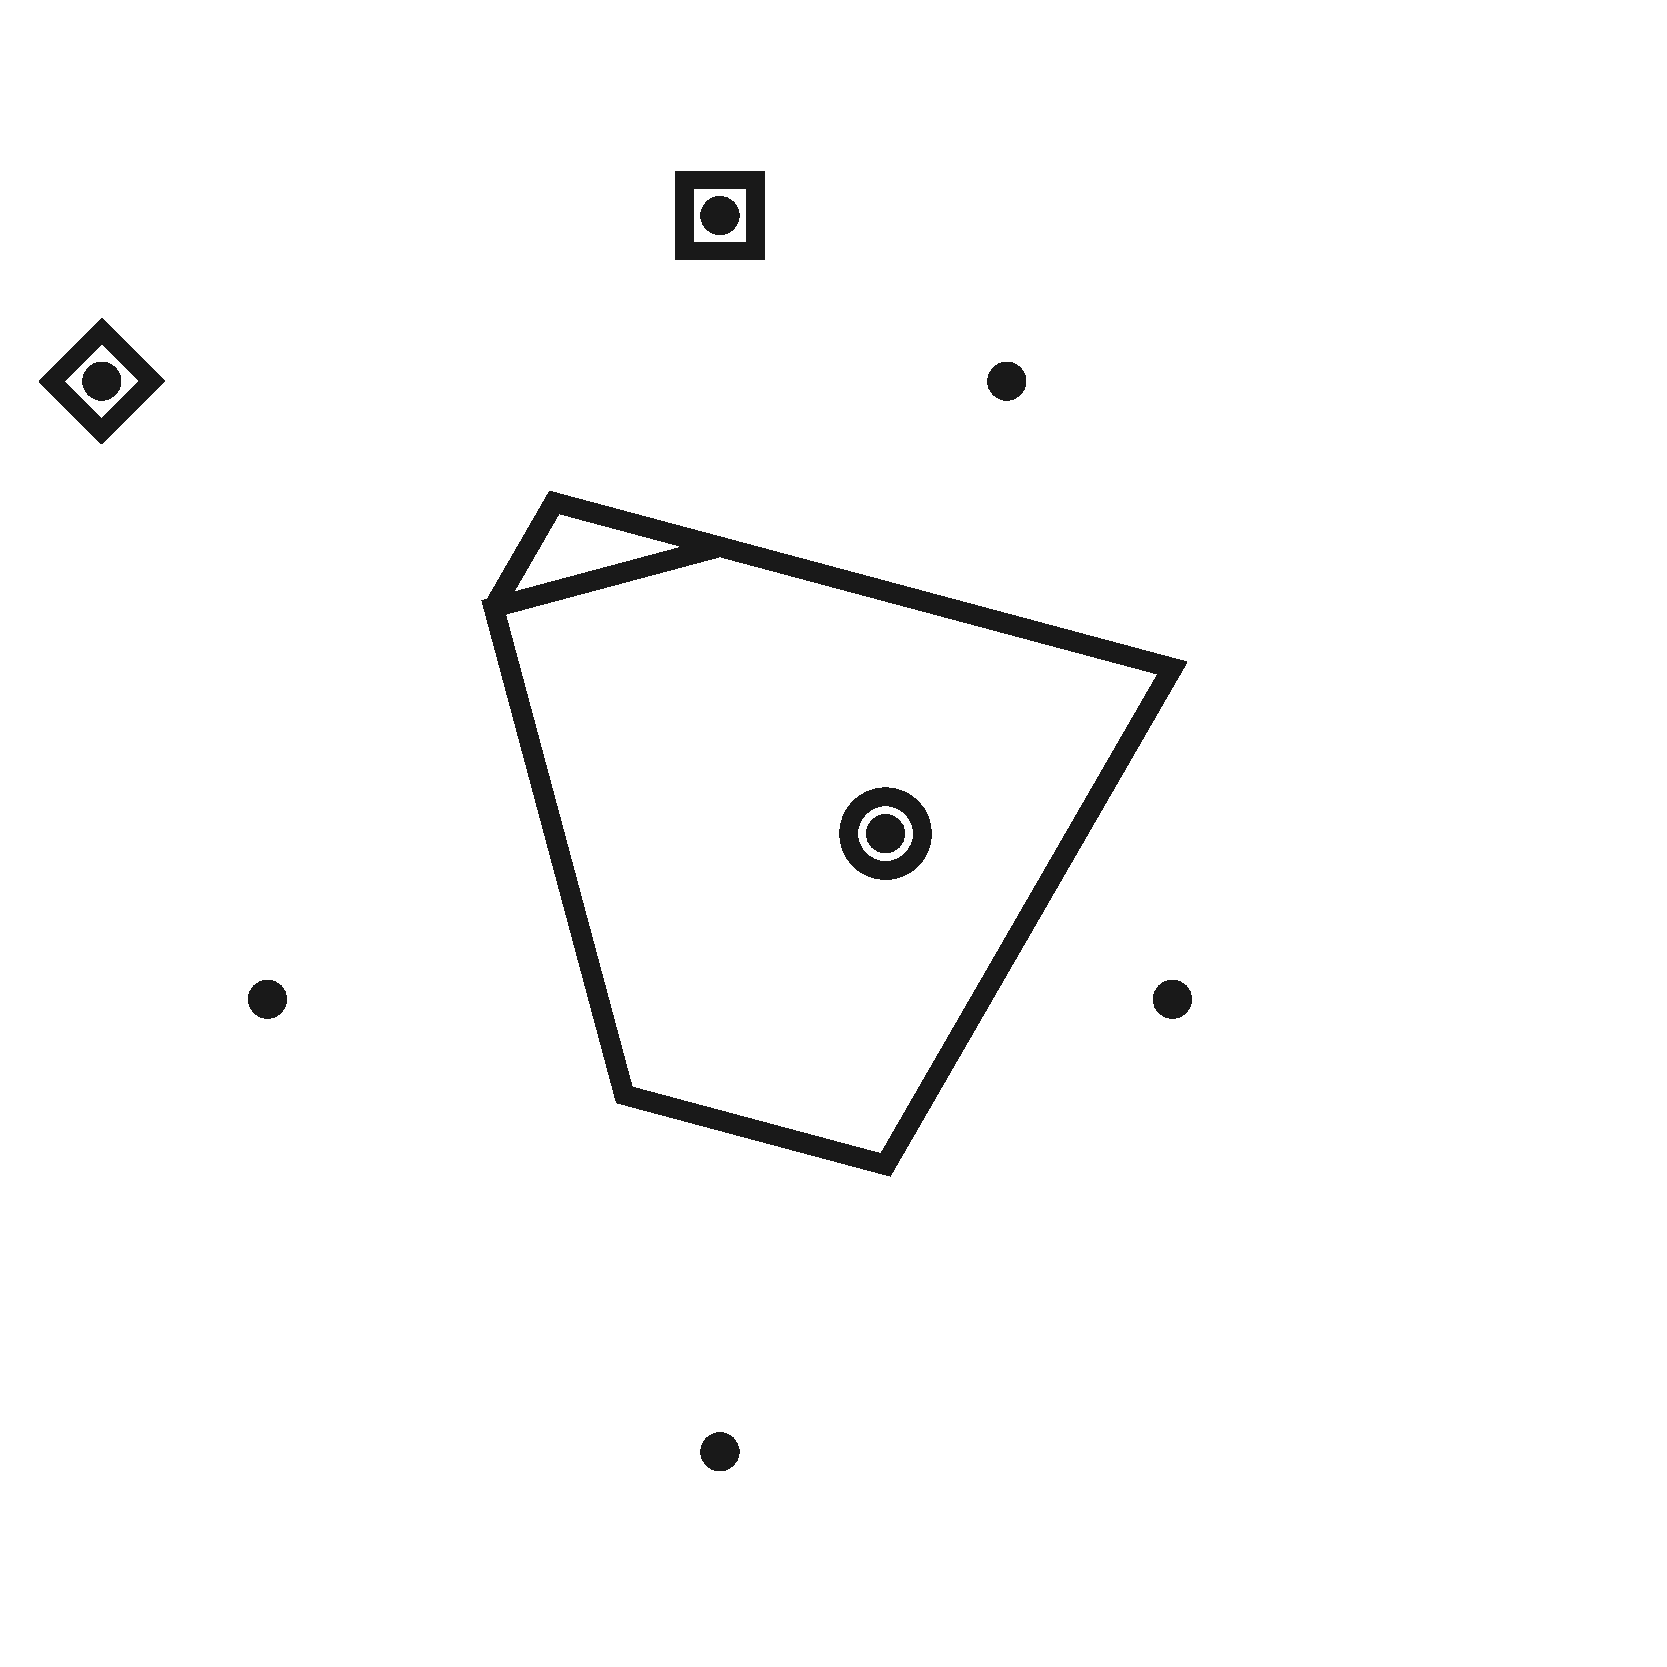
\includegraphics[scale=0.11]{catalogRhombusAll/tiles/tile003}%
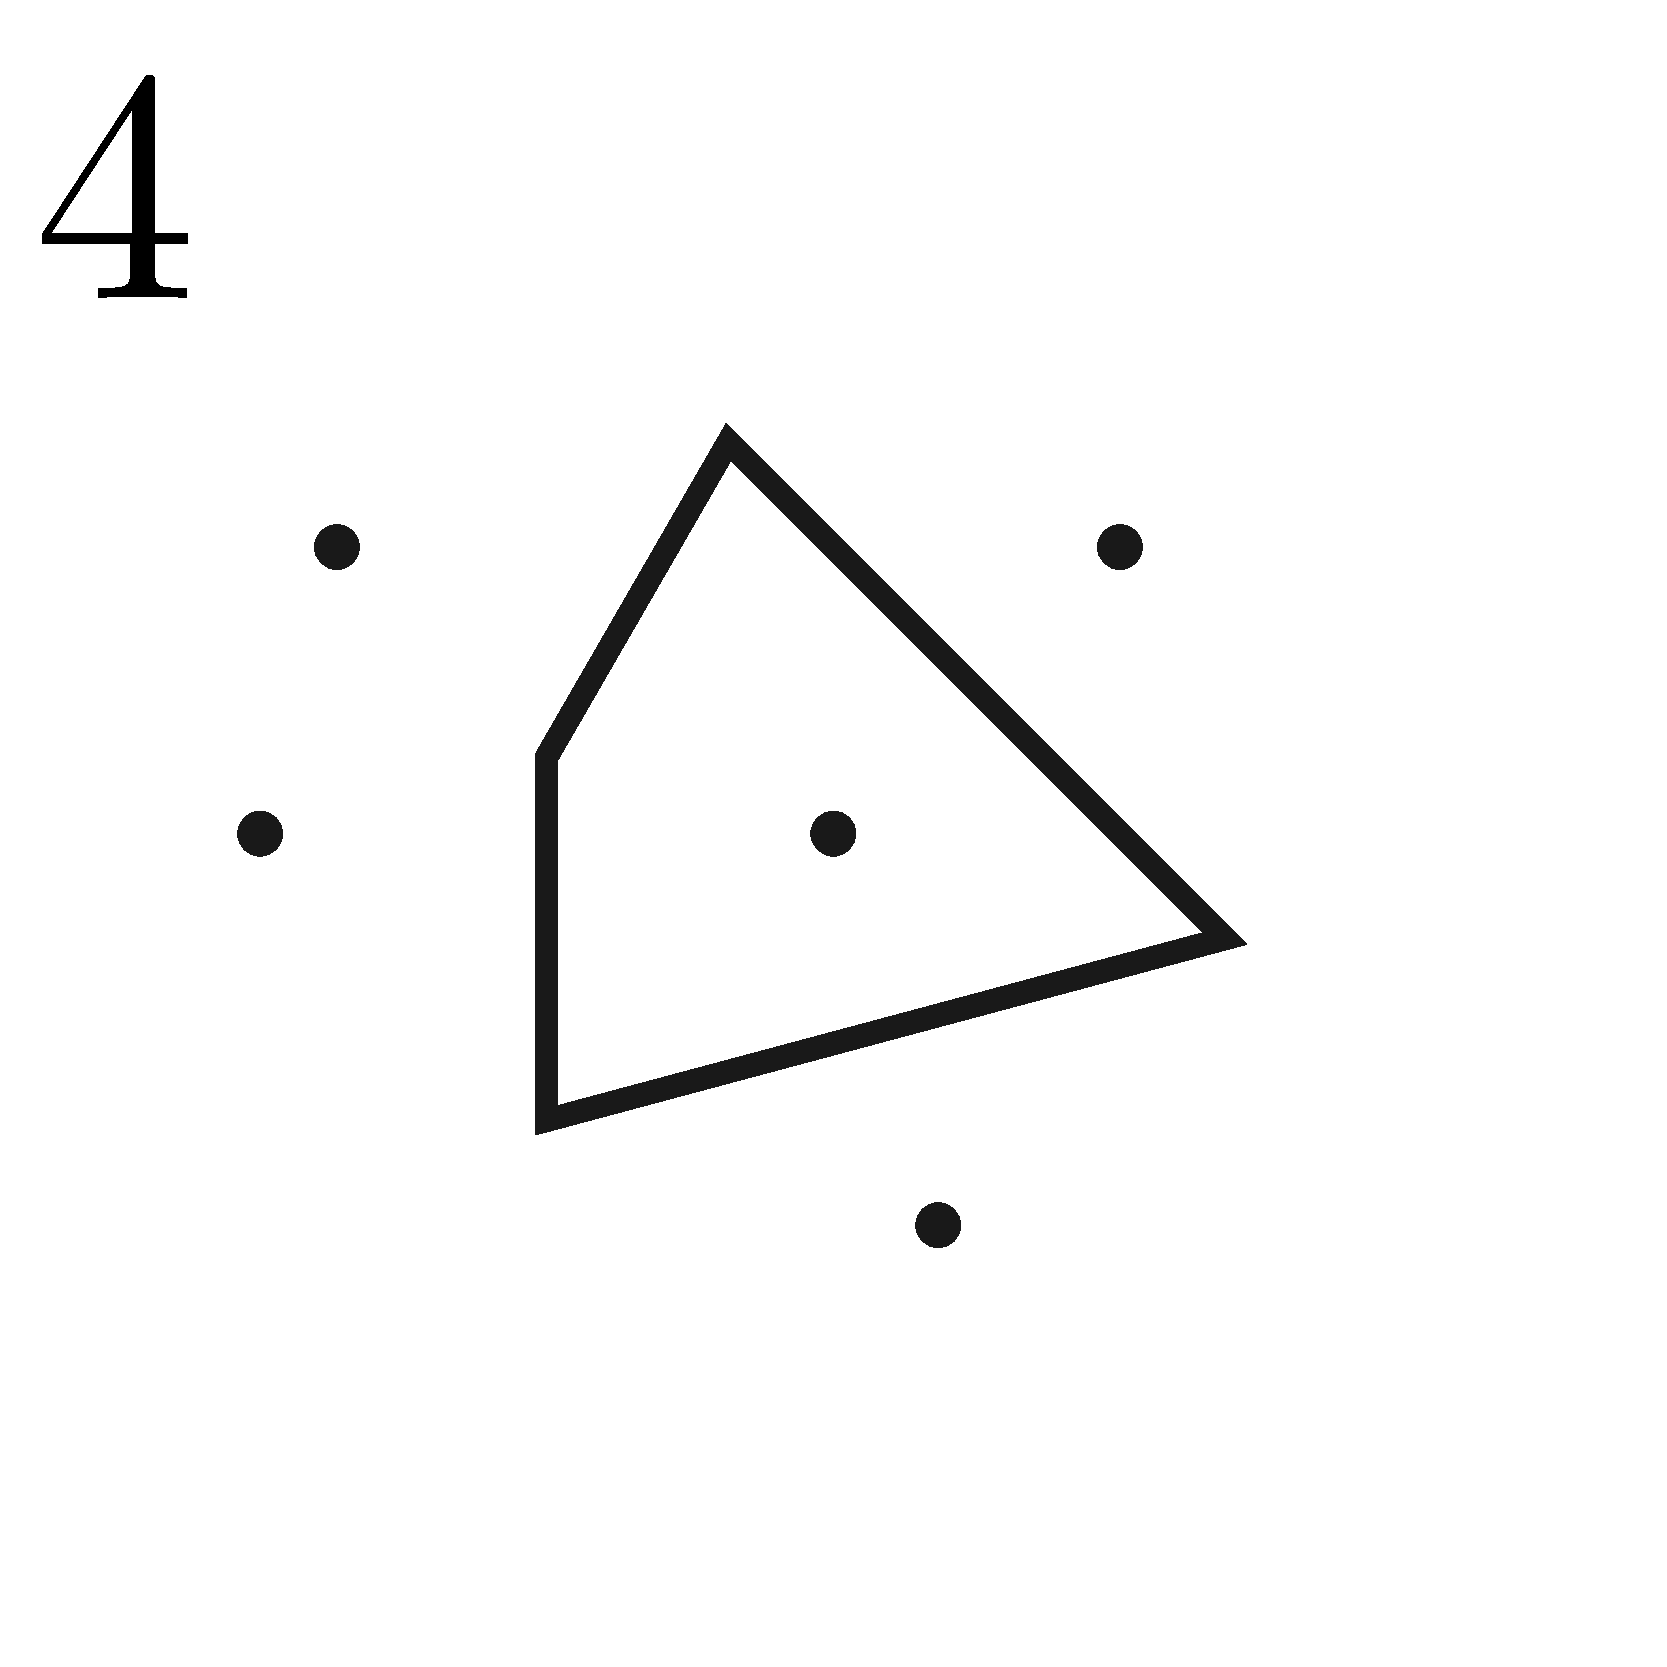
\includegraphics[scale=0.11]{catalogRhombusAll/tiles/tile004}%
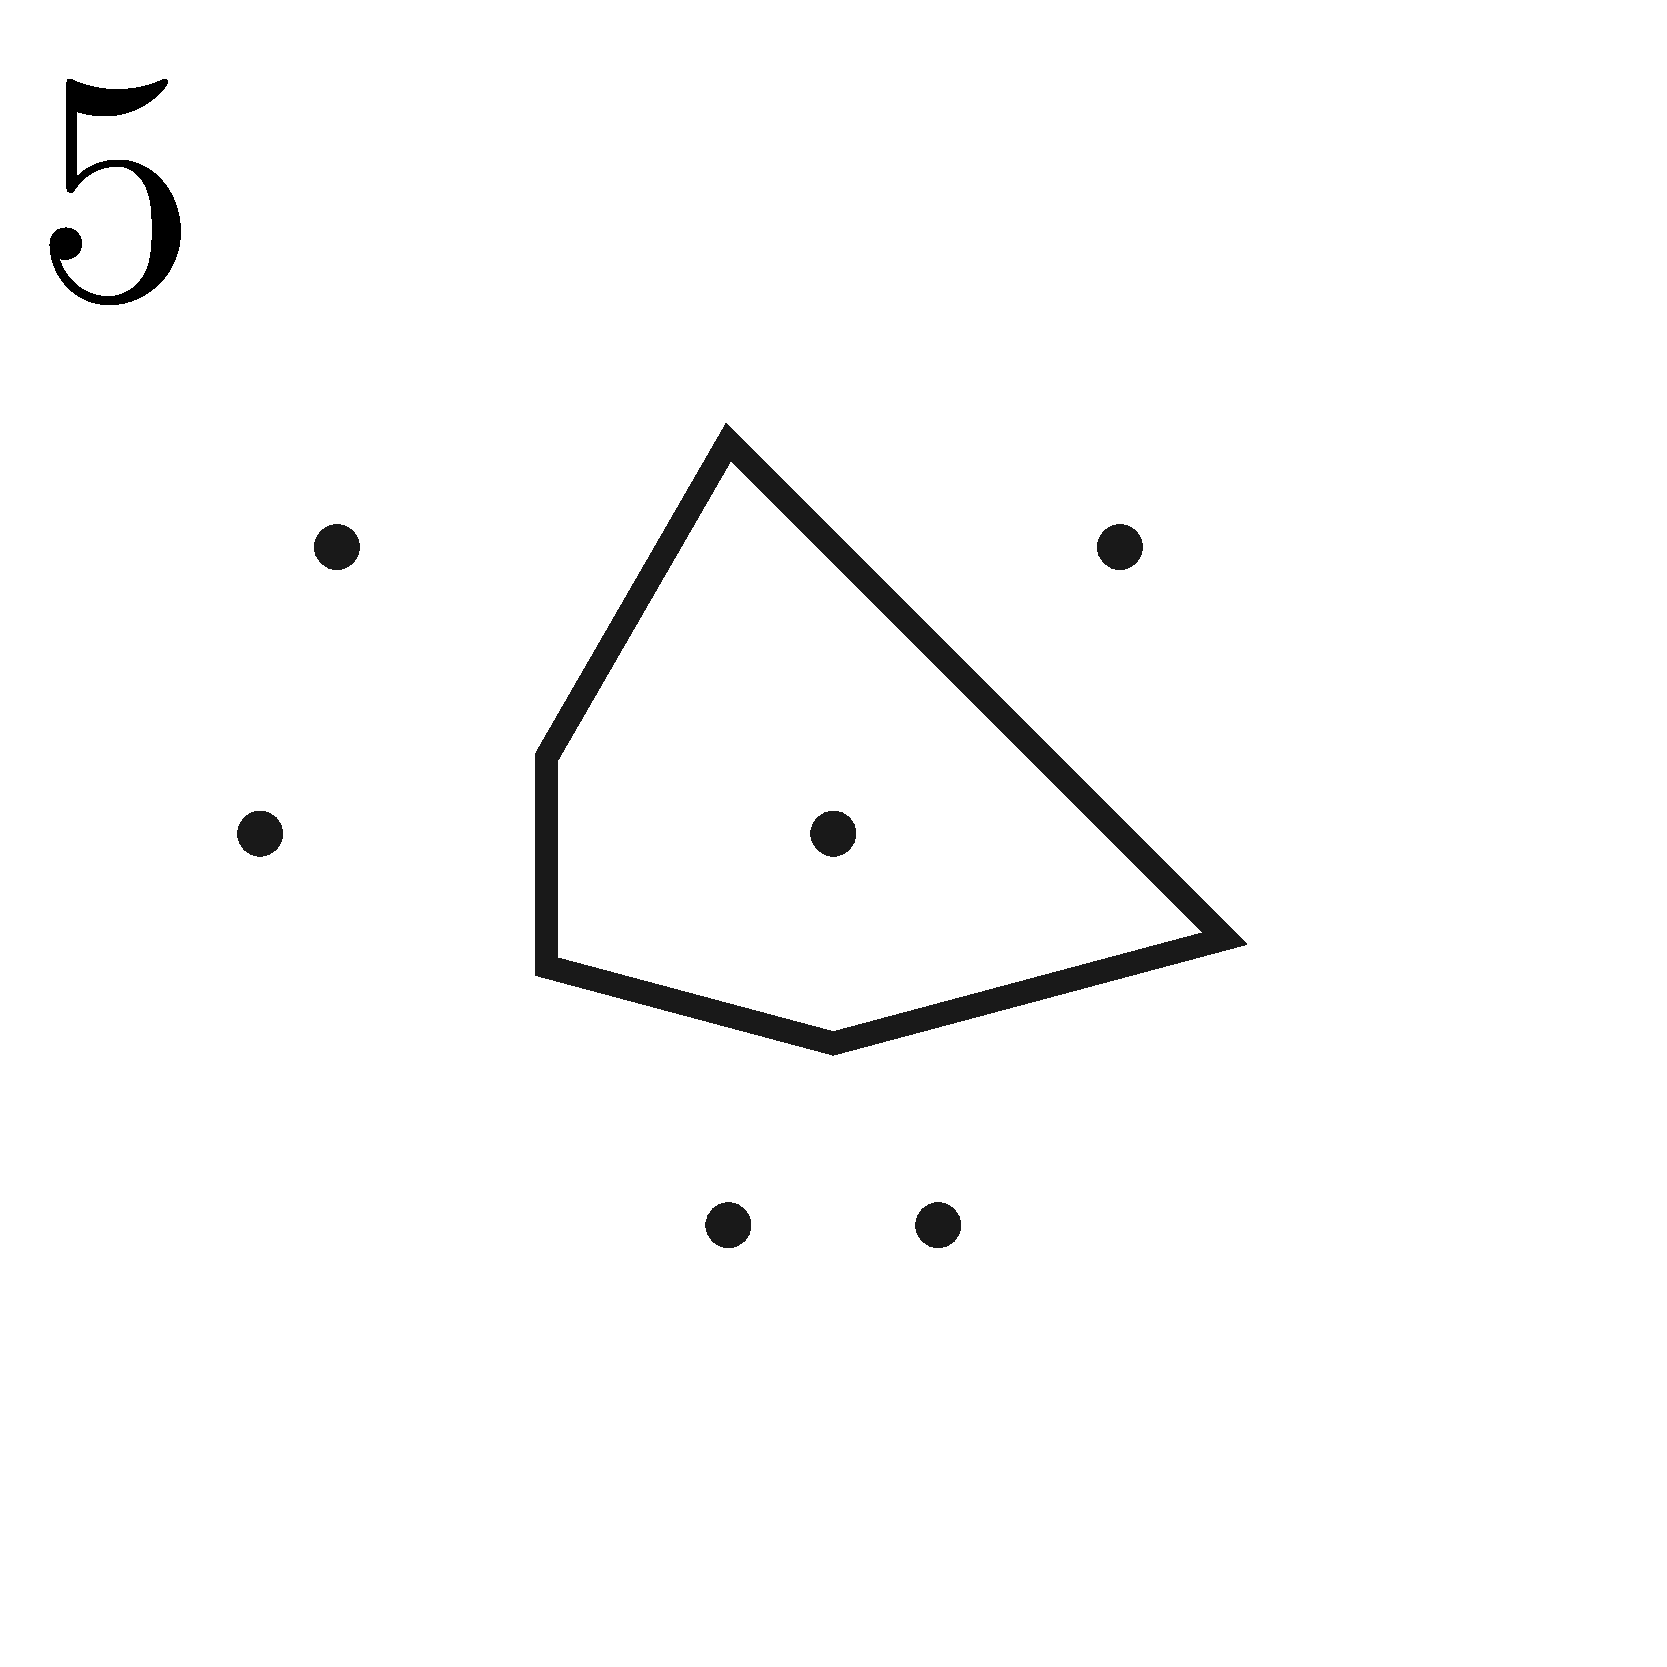
\includegraphics[scale=0.11]{catalogRhombusAll/tiles/tile005}%
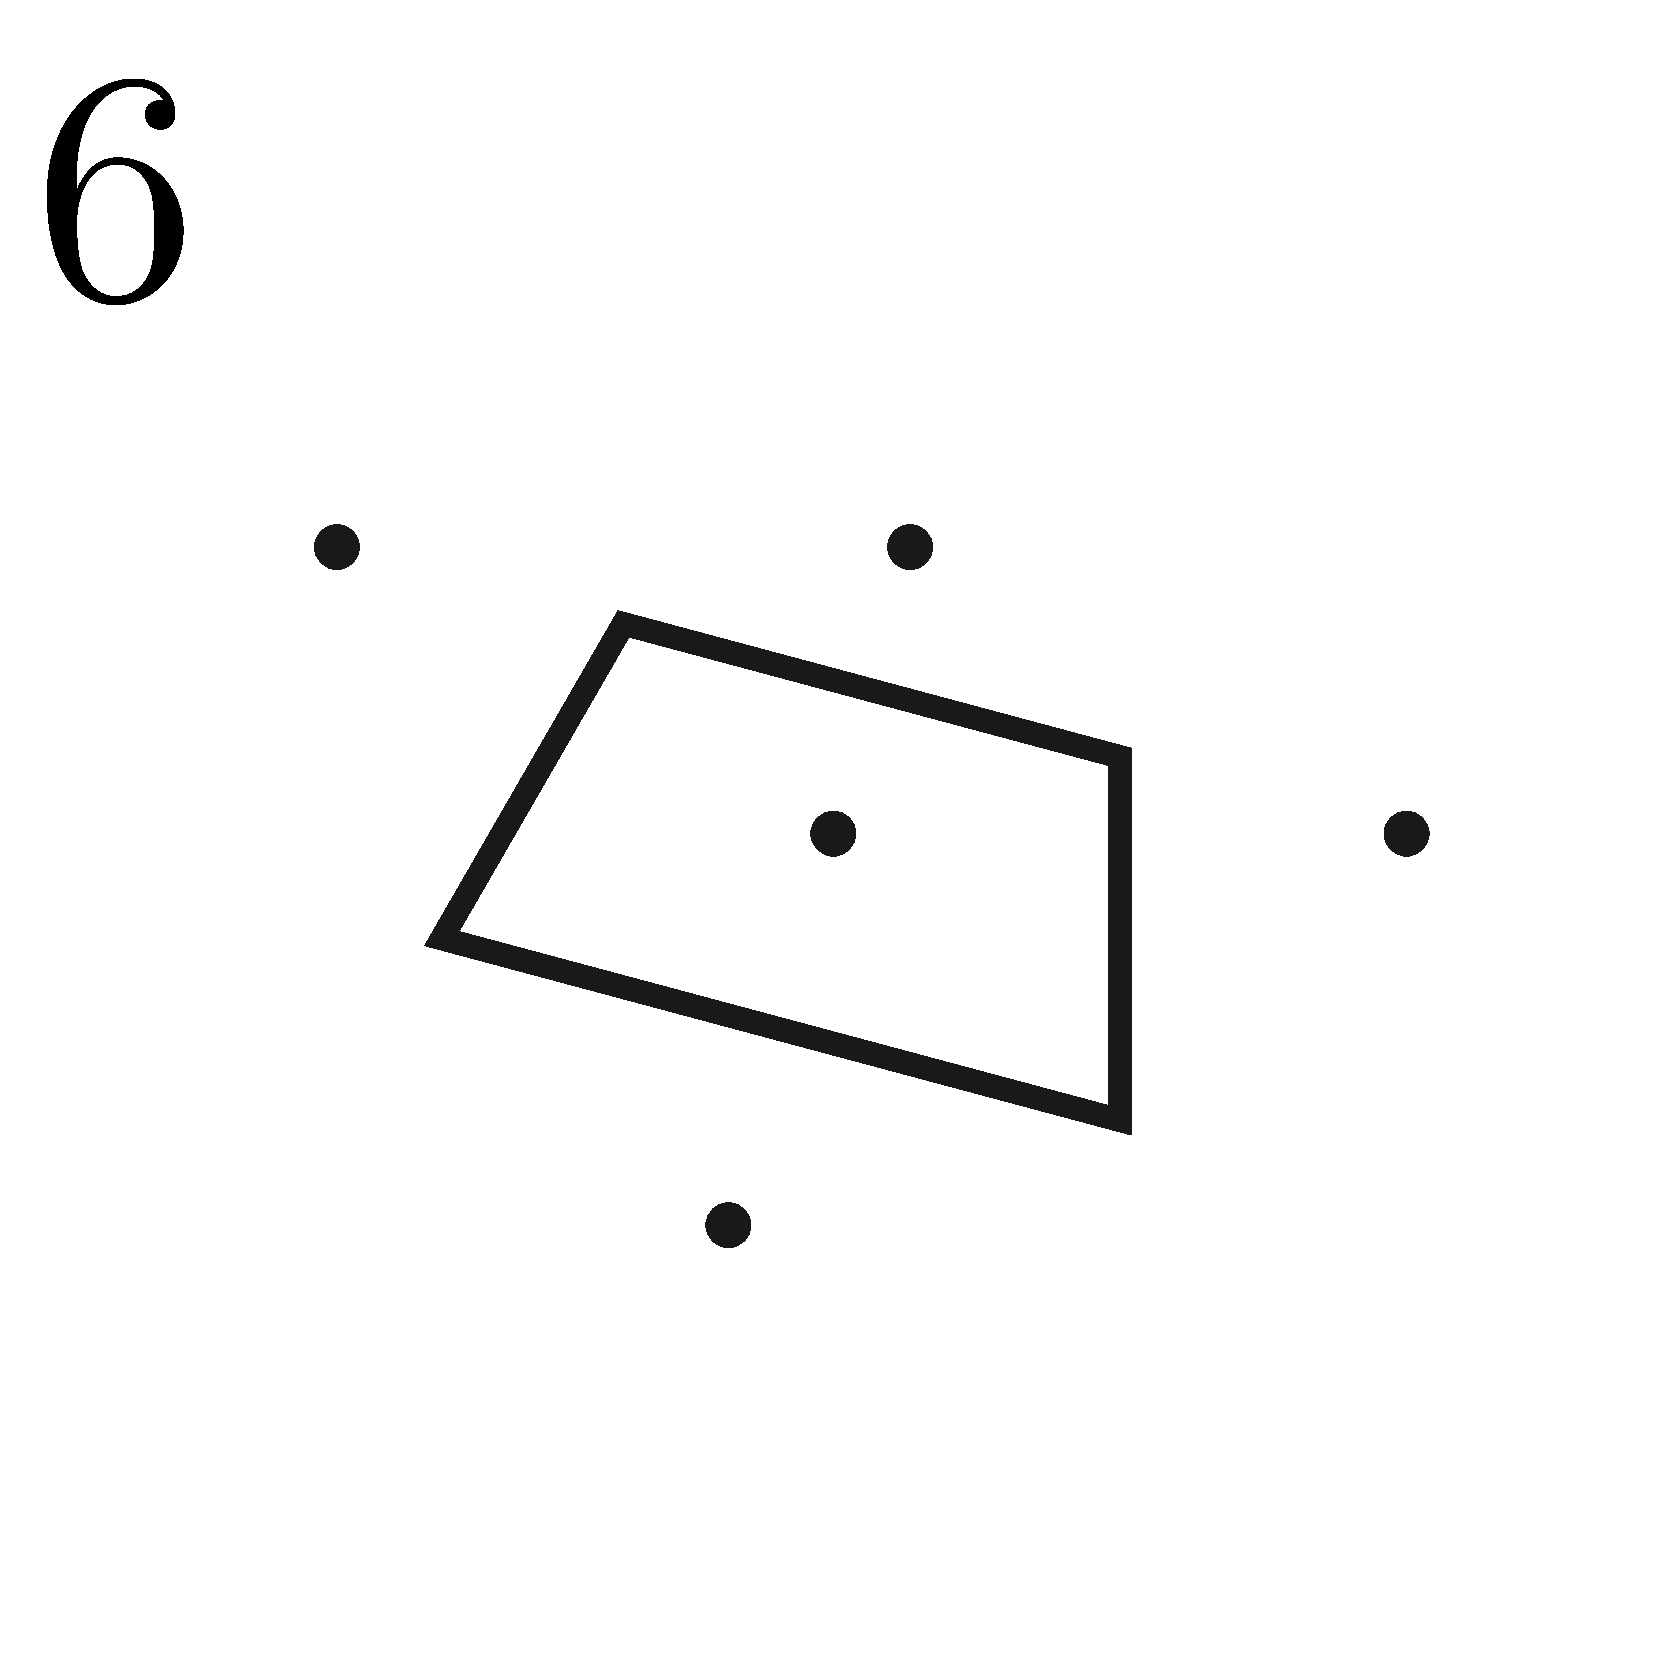
\includegraphics[scale=0.11]{catalogRhombusAll/tiles/tile006}
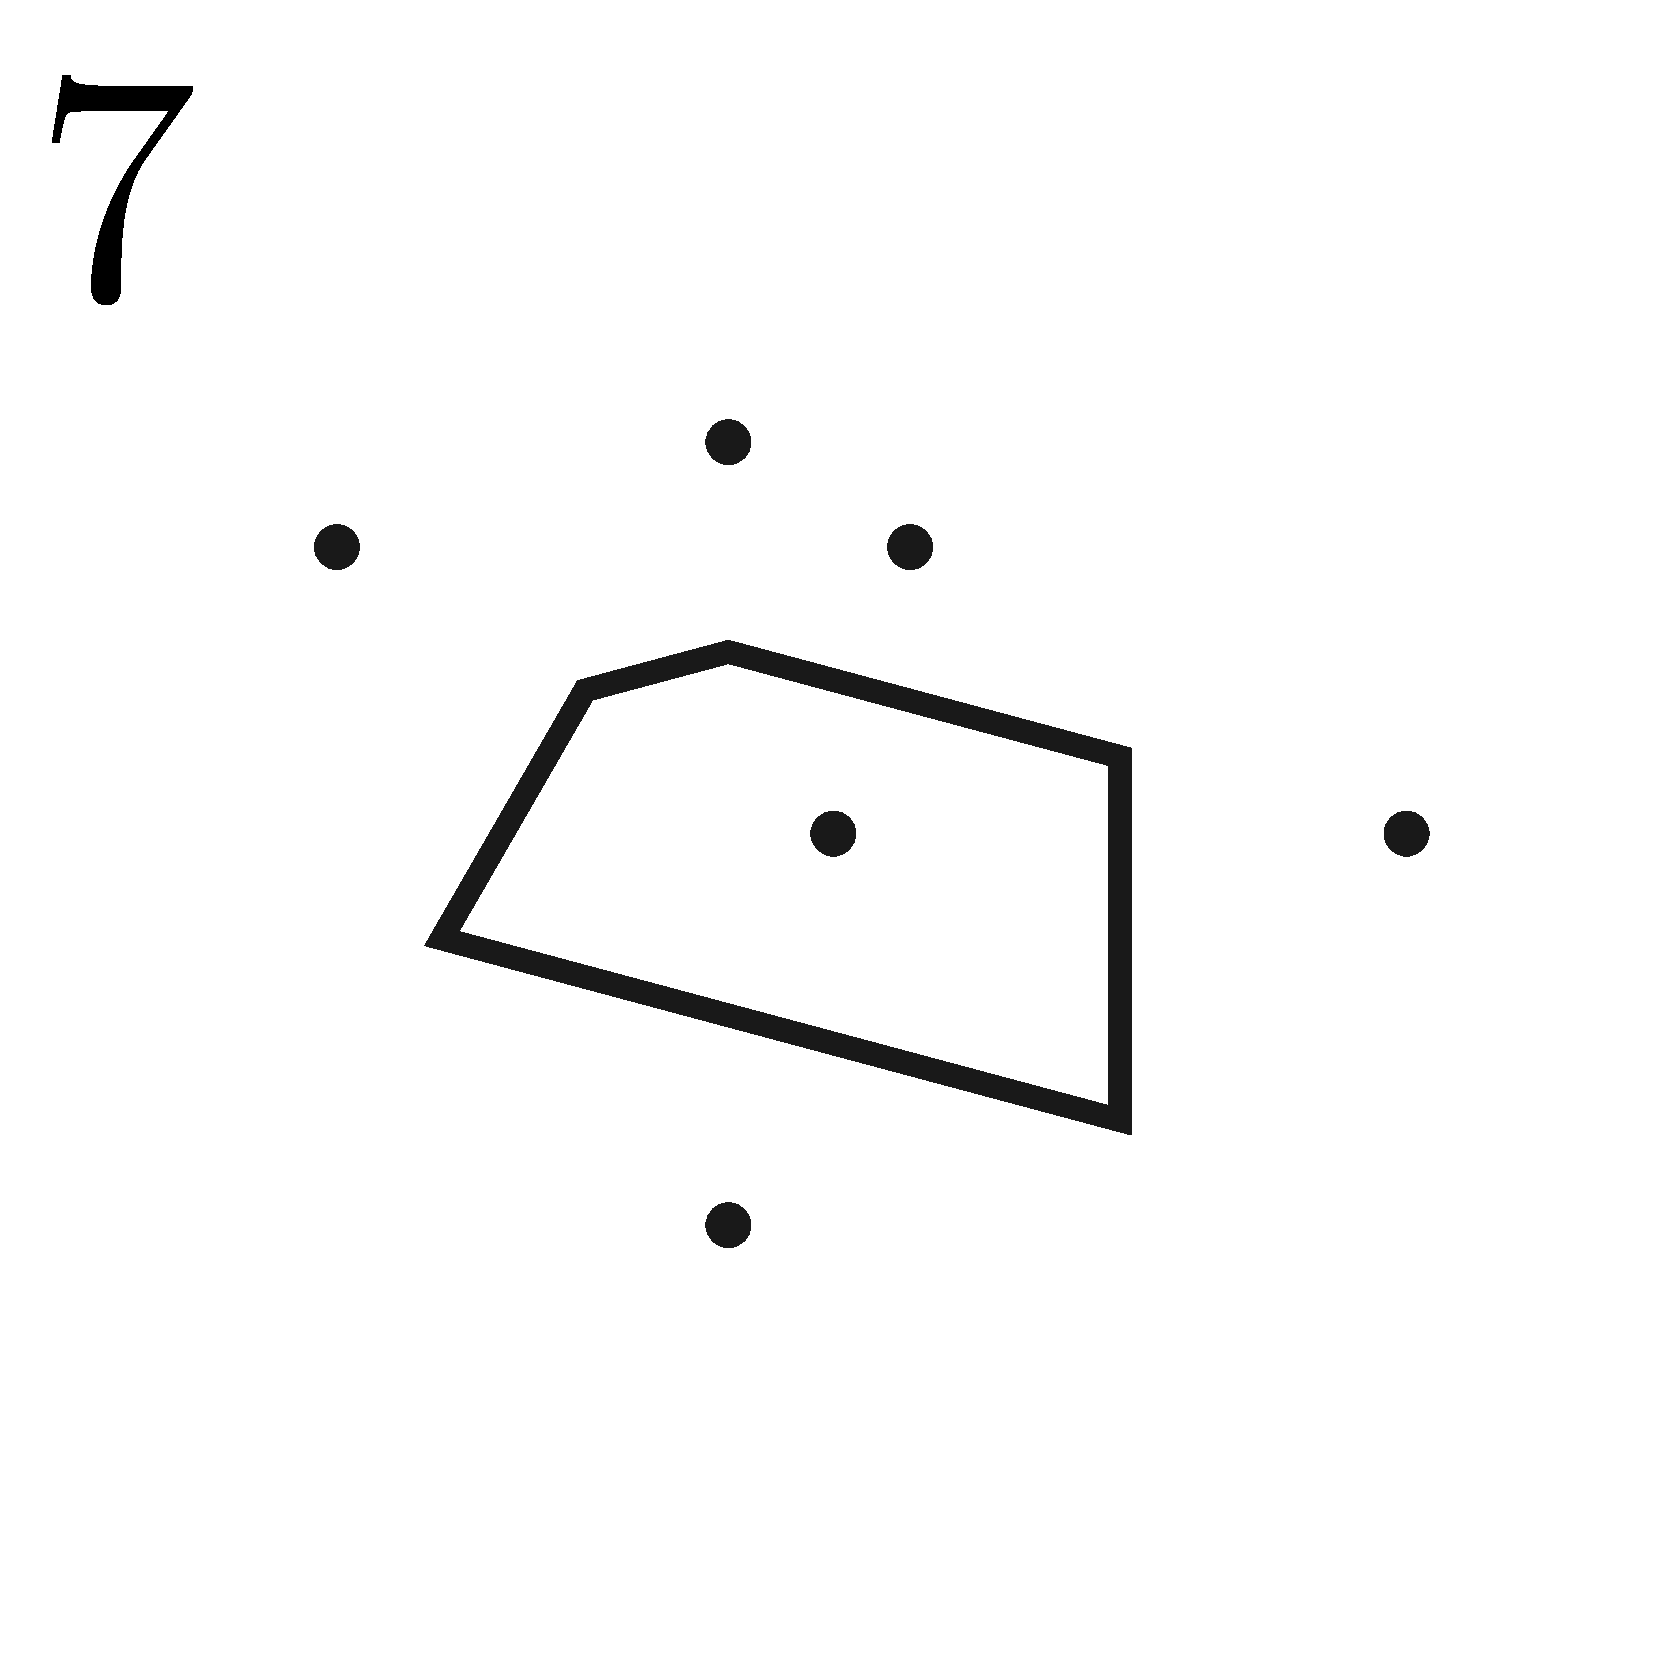
\includegraphics[scale=0.11]{catalogRhombusAll/tiles/tile007}%
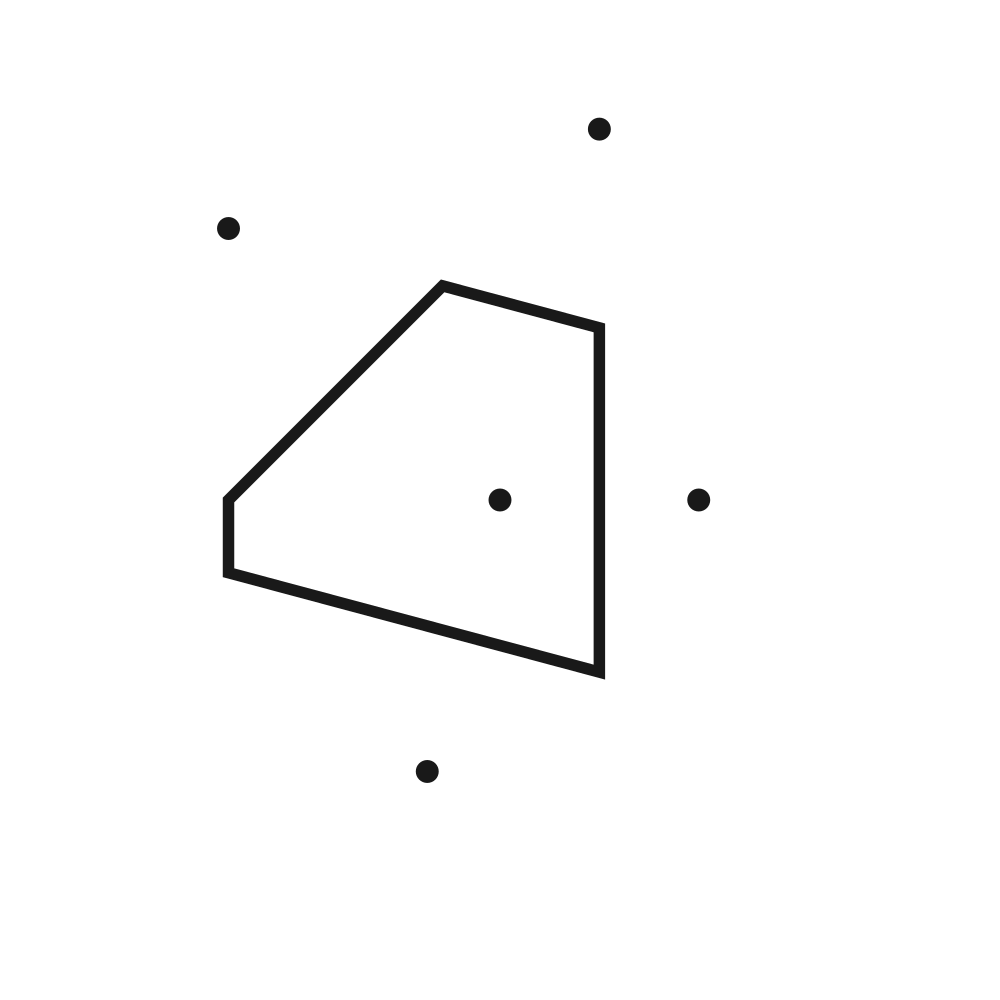
\includegraphics[scale=0.11]{catalogRhombusAll/tiles/tile008}%
\includegraphics[scale=0.11]{catalogRhombusAll/tiles/tile009}%
\includegraphics[scale=0.11]{catalogRhombusAll/tiles/tile010}%
\includegraphics[scale=0.11]{catalogRhombusAll/tiles/tile011}%
\includegraphics[scale=0.11]{catalogRhombusAll/tiles/tile012}
\includegraphics[scale=0.11]{catalogRhombusAll/tiles/tile013}%
\includegraphics[scale=0.11]{catalogRhombusAll/tiles/tile014}%
\includegraphics[scale=0.11]{catalogRhombusAll/tiles/tile015}%
\includegraphics[scale=0.11]{catalogRhombusAll/tiles/tile016}%
\includegraphics[scale=0.11]{catalogRhombusAll/tiles/tile017}%
\includegraphics[scale=0.11]{catalogRhombusAll/tiles/tile018}
\includegraphics[scale=0.11]{catalogRhombusAll/tiles/tile019}%
\includegraphics[scale=0.11]{catalogRhombusAll/tiles/tile020}%
\includegraphics[scale=0.11]{catalogRhombusAll/tiles/tile021}%
\includegraphics[scale=0.11]{catalogRhombusAll/tiles/tile022}%
\includegraphics[scale=0.11]{catalogRhombusAll/tiles/tile023}%
\includegraphics[scale=0.11]{catalogRhombusAll/tiles/tile024}
\includegraphics[scale=0.11]{catalogRhombusAll/tiles/tile025}%
\includegraphics[scale=0.11]{catalogRhombusAll/tiles/tile026}%
\includegraphics[scale=0.11]{catalogRhombusAll/tiles/tile027}%
\includegraphics[scale=0.11]{catalogRhombusAll/tiles/tile028}%
\includegraphics[scale=0.11]{catalogRhombusAll/tiles/tile029}%
\includegraphics[scale=0.11]{catalogRhombusAll/tiles/tile030}
\includegraphics[scale=0.11]{catalogRhombusAll/tiles/tile031}%
\includegraphics[scale=0.11]{catalogRhombusAll/tiles/tile032}%
\includegraphics[scale=0.11]{catalogRhombusAll/tiles/tile033}%
\includegraphics[scale=0.11]{catalogRhombusAll/tiles/tile034}%
\includegraphics[scale=0.11]{catalogRhombusAll/tiles/tile035}%
\includegraphics[scale=0.11]{catalogRhombusAll/tiles/tile036}
\includegraphics[scale=0.11]{catalogRhombusAll/tiles/tile037}%
\includegraphics[scale=0.11]{catalogRhombusAll/tiles/tile038}%
\includegraphics[scale=0.11]{catalogRhombusAll/tiles/tile039}%
\includegraphics[scale=0.11]{catalogRhombusAll/tiles/tile040}%
\includegraphics[scale=0.11]{catalogRhombusAll/tiles/tile041}%
\includegraphics[scale=0.11]{catalogRhombusAll/tiles/tile042}
\includegraphics[scale=0.11]{catalogRhombusAll/tiles/tile043}%
\includegraphics[scale=0.11]{catalogRhombusAll/tiles/tile044}%
\includegraphics[scale=0.11]{catalogRhombusAll/tiles/tile045}%
\includegraphics[scale=0.11]{catalogRhombusAll/tiles/tile046}%
\includegraphics[scale=0.11]{catalogRhombusAll/tiles/tile047}%
\includegraphics[scale=0.11]{catalogRhombusAll/tiles/tile048}
\includegraphics[scale=0.11]{catalogRhombusAll/tiles/tile049}%
\includegraphics[scale=0.11]{catalogRhombusAll/tiles/tile050}%
\includegraphics[scale=0.11]{catalogRhombusAll/tiles/tile051}%
\includegraphics[scale=0.11]{catalogRhombusAll/tiles/tile052}%
\includegraphics[scale=0.11]{catalogRhombusAll/tiles/tile053}%
\end{flushleft}
\end{figure}


\begin{table}
\centering
\rowcolors{1}{white}{gray!20}
\begin{tabular}{l|ccccccccccccccccccccc}
	\toprule
		& $1$ 	    & $2$       & $3$       & $4$       & $5$       & $6$       & $7$       & $8$       & $9$       & $10$      & $11$      & $12$      & $13$      & $14$      & $15$      & $16$      & $17$      & $18$      & $19$      & $20$      & $21$      \\ 
	\midrule
1	  & $\bullet$	& $\bullet$ & $\bullet$ & $\bullet$	&           &           &           &           &           &           &           &           &           &           &           &           &           &           &           &           &           \\
2   & $\bullet$ & $\bullet$ & $\bullet$ & $\bullet$ & $\bullet$ & $\bullet$ & $\bullet$ & $\bullet$ &           &           &           &           &           &           &           &           &           &           &           &           &           \\
3   &           & $\bullet$ & $\bullet$ & $\bullet$ &           &           &           &           &           &           &           &           &           &           &           &           &           &           &           &           &           \\
4   & $\bullet$ & $\bullet$ & $\bullet$ & $\bullet$ &           &           &           &           &           &           &           &           &           &           &           &           &           &           &           &           &           \\
5   &           & $\bullet$ & $\bullet$ & $\bullet$ &           &           &           &           &           &           &           &           &           &           &           &           &           &           &           &           &           \\
6   & $\bullet$ & $\bullet$ & $\bullet$ & $\bullet$ & $\bullet$ & $\bullet$ & $\bullet$ & $\bullet$ &           &           &           &           &           &           &           &           &           &           &           &           &           \\
7   &           & $\bullet$ & $\bullet$ & $\bullet$ & $\bullet$ & $\bullet$ &           &           &           &           &           &           &           &           &           &           &           &           &           &           &           \\
8   &           & $\bullet$ & $\bullet$ & $\bullet$ &           &           &           &           &           &           &           &           &           &           &           &           &           &           &           &           &           \\
9   &           & $\bullet$ & $\bullet$ & $\bullet$ & $\bullet$ & $\bullet$ & $\bullet$ & $\bullet$ &           &           &           &           &           &           &           &           &           &           &           &           &           \\
10  &           & $\bullet$ & $\bullet$ & $\bullet$ & $\bullet$ & $\bullet$ & $\bullet$ & $\bullet$ & $\bullet$ & $\bullet$ &           &           &           &           &           &           &           &           &           &           &           \\
11  &           &           &           &           &           &           &           & $\bullet$ &           &           &           &           &           &           &           &           &           &           &           &           &           \\
12  &           & $\bullet$ & $\bullet$ & $\bullet$ & $\bullet$ & $\bullet$ & $\bullet$ & $\bullet$ & $\bullet$ & $\bullet$ & $\bullet$ & $\bullet$ & $\bullet$ & $\bullet$ &           &           &           &           &           &           &           \\
13  &           &           &           &           &           & $\bullet$ &           &           &           &           &           &           &           &           &           &           &           &           &           &           &           \\
14  &           & $\bullet$ & $\bullet$ & $\bullet$ &           &           &           &           &           &           &           &           &           &           &           &           &           &           &           &           &           \\
15  &           &           &           &           &           &           &           & $\bullet$ & $\bullet$ & $\bullet$ &           &           &           &           &           &           &           &           &           &           &           \\
16  &           &           &           &           &           &           &           & $\bullet$ &           &           &           &           &           &           &           &           &           &           &           &           &           \\
17  &           & $\bullet$ & $\bullet$ & $\bullet$ & $\bullet$ & $\bullet$ & $\bullet$ & $\bullet$ &           &           &           &           &           &           &           &           &           &           &           &           &           \\
18  &           &           &           &           &           & $\bullet$ & $\bullet$ & $\bullet$ &           &           &           &           &           &           &           &           &           &           &           &           &           \\
19  &           &           &           &           &           &           &           &           &           &           &           & $\bullet$ & $\bullet$ & $\bullet$ & $\bullet$ & $\bullet$ & $\bullet$ & $\bullet$ & $\bullet$ & $\bullet$ &           \\
20  &           & $\bullet$ & $\bullet$ & $\bullet$ & $\bullet$ & $\bullet$ &           &           &           &           &           &           &           &           &           &           &           &           &           &           &           \\
21  &           &           &           &           &           & $\bullet$ & $\bullet$ & $\bullet$ & $\bullet$ & $\bullet$ &           &           &           &           &           &           &           &           &           &           &           \\
22  &           &           &           &           &           &           &           & $\bullet$ & $\bullet$ & $\bullet$ &           &           &           &           &           &           &           &           &           &           &           \\
23  &           &           &           &           &           &           &           & $\bullet$ & $\bullet$ & $\bullet$ &           &           &           &           &           &           &           &           &           &           &           \\
24  &           &           &           &           &           & $\bullet$ & $\bullet$ & $\bullet$ & $\bullet$ & $\bullet$ & $\bullet$ & $\bullet$ &           &           &           &           &           &           &           &           &           \\
25  &           &           &           &           &           &           &           &           &           & $\bullet$ &           &           &           &           &           &           &           &           &           &           &           \\
26  &           &           &           &           &           &           &           &           &           & $\bullet$ &           &           &           &           &           &           &           &           &           &           &           \\
27  &           &           &           &           &           &           &           &           &           & $\bullet$ & $\bullet$ & $\bullet$ &           &           &           &           &           &           &           &           &           \\
28  &           &           &           &           &           &           &           &           &           & $\bullet$ & $\bullet$ & $\bullet$ & $\bullet$ & $\bullet$ &           &           &           &           &           &           &           \\
29  &           &           &           &           &           &           &           &           &           & $\bullet$ &           &           &           &           &           &           &           &           &           &           &           \\
30  &           &           &           &           &           &           &           &           &           & $\bullet$ & $\bullet$ & $\bullet$ & $\bullet$ & $\bullet$ &           &           &           &           &           &           &           \\
31  &           &           &           &           &           &           &           &           &           & $\bullet$ & $\bullet$ & $\bullet$ &           &           &           &           &           &           &           &           &           \\
32  &           &           &           &           &           &           &           &           &           &           &           &           &           & $\bullet$ &           &           &           &           &           &           &           \\
33  &           &           &           &           &           &           &           &           &           &           &           & $\bullet$ & $\bullet$ & $\bullet$ &           &           &           &           &           &           &           \\
34  &           &           &           &           &           &           &           &           &           &           &           & $\bullet$ &           &           &           &           &           &           &           &           &           \\
35  &           &           &           &           &           &           &           &           &           & $\bullet$ & $\bullet$ & $\bullet$ & $\bullet$ & $\bullet$ &           &           &           &           &           &           &           \\
36  &           &           &           &           &           &           &           &           &           &           &           &           &           & $\bullet$ & $\bullet$ & $\bullet$ &           &           &           &           &           \\
37  &           &           &           &           &           &           &           &           &           &           &           &           &           & $\bullet$ & $\bullet$ &           &           &           &           &           &           \\
38  &           & $\bullet$ & $\bullet$ & $\bullet$ & $\bullet$ & $\bullet$ &           &           &           &           &           &           &           &           &           &           &           &           &           &           &           \\
39  &           &           &           &           &           &           &           &           &           &           &           & $\bullet$ & $\bullet$ & $\bullet$ & $\bullet$ &           &           &           &           &           &           \\
40  &           &           &           &           &           &           &           &           &           & $\bullet$ & $\bullet$ & $\bullet$ & $\bullet$ & $\bullet$ &           &           &           &           &           &           &           \\
41  &           &           &           &           &           &           &           &           &           &           &           &           &           & $\bullet$ & $\bullet$ & $\bullet$ &           &           &           &           &           \\
42  &           &           &           &           &           &           &           &           &           &           &           & $\bullet$ & $\bullet$ & $\bullet$ &           &           &           &           &           &           &           \\ 
43  &           &           &           &           &           &           &           &           &           &           &           & $\bullet$ & $\bullet$ & $\bullet$ & $\bullet$ & $\bullet$ & $\bullet$ & $\bullet$ & $\bullet$ & $\bullet$ &           \\
44  &           &           &           &           &           & $\bullet$ & $\bullet$ & $\bullet$ &           &           &           &           &           &           &           &           &           &           &           &           &           \\
45  &           &           &           &           &           &           &           &           &           & $\bullet$ & $\bullet$ & $\bullet$ & $\bullet$ & $\bullet$ & $\bullet$ & $\bullet$ & $\bullet$ & $\bullet$ & $\bullet$ & $\bullet$ &           \\
46  &           &           &           &           &           &           &           &           &           &           &           &           &           &           &           &           &           & $\bullet$ & $\bullet$ & $\bullet$ &           \\ 
47  &           &           &           &           &           &           &           &           &           &           &           &           &           &           &           & $\bullet$ & $\bullet$ & $\bullet$ & $\bullet$ & $\bullet$ &           \\
48  &           &           &           &           &           &           &           &           &           &           &           &           &           &           &           & $\bullet$ & $\bullet$ & $\bullet$ & $\bullet$ & $\bullet$ &           \\ 
49  &           &           &           &           &           &           &           &           &           &           &           &           &           &           &           & $\bullet$ & $\bullet$ & $\bullet$ & $\bullet$ & $\bullet$ &           \\
50  &           &           &           &           &           &           &           &           &           &           &           & $\bullet$ & $\bullet$ & $\bullet$ & $\bullet$ & $\bullet$ & $\bullet$ & $\bullet$ & $\bullet$ & $\bullet$ & $\bullet$ \\ 
51  &           &           &           &           &           &           &           &           &           &           &           &           &           &           &           & $\bullet$ & $\bullet$ & $\bullet$ & $\bullet$ & $\bullet$ & $\bullet$ \\
52  &           &           &           &           &           &           &           &           &           &           &           &           &           &           &           & $\bullet$ & $\bullet$ & $\bullet$ & $\bullet$ & $\bullet$ & $\bullet$ \\
53  &           &           &           &           &           &           &           &           &           &           &           &           &           &           &           & $\bullet$ & $\bullet$ & $\bullet$ & $\bullet$ & $\bullet$ & $\bullet$ \\
\bottomrule
\end{tabular}
\caption{Assignment of voronoi polygons to their quasicrystals. Horizontal axis enumerates members of $\mathcal{D}$ and the vertical axis corresponds to the numbers from the list of voronoi polygons.}
\label{table:tiles1}
\end{table}

\restoregeometry

\end{document}
